\documentclass[letterpaper]{article} 
\usepackage[left = 0.5in, right = 0.5in, top = 0.9in, bottom = 0.9in]{geometry}
\usepackage{enumitem}
\usepackage{multicol}
\usepackage[spanish]{babel}
\usepackage[utf8]{inputenc}

\usepackage{amsmath,amssymb,amsthm}
\usepackage{tikz-cd}
\usepackage{mathrsfs}
\usepackage[bbgreekl]{mathbbol}
\usepackage{dsfont}
\usepackage{graphicx}
\graphicspath{{img/}}

\newcommand{\op}{\operatorname}
\newcommand{\Op}{^{\op{op}}}
\newcommand{\scc}{\mathscr C}
\newcommand{\scd}{\mathscr D}
\newcommand{\sce}{\mathscr E}
\newcommand{\sci}{\mathscr I}
\newcommand{\scj}{\mathscr J}
\newcommand{\scx}{\mathscr X}
\newcommand{\var}{\mathrm{Var}}
\newcommand{\Id}{\operatorname{Id}}
\newcommand{\N}{\mathbb N}
\newcommand{\Z}{\mathbb Z}
\newcommand{\Q}{\mathbb{Q}}
\newcommand{\I}{\mathbb{I}}
\newcommand{\R}{\mathbb{R}}
\newcommand{\C}{\mathbb{C}}
\newcommand{\F}{\mathcal{F}}
\newcommand{\G}{\mathcal{G}}
\newcommand{\B}{\mathcal{B}}
\newcommand{\abs}[1]{\left\lvert #1 \right\rvert}
\newcommand{\inv}{^{-1}}
\renewcommand{\to}{\rightarrow}
\newcommand{\ent}{\Longrightarrow}
\newcommand{\E}{\mathbb{E}}
\renewcommand{\P}{\mathbb{P}}
\newcommand{\1}{\mathds{1}}
\renewcommand{\qedsymbol}{$\blacksquare$}

\theoremstyle{definition}
\newtheorem{dfn}{Definición}
\theoremstyle{definition}
\newtheorem{teo}{Teorema}
\theoremstyle{definition}
\newtheorem{cor}{Corolario}
\theoremstyle{definition}
\newtheorem{prop}{Proposición}
\theoremstyle{definition}
\newtheorem{obs}{Observación}


\title{\textbf{Cómputo Científico\\
Tarea 8\\
MCMC: MH con Kérneles Híbridos y Gibbs Sampler}}
\author{Iván Irving Rosas Domínguez}
\date{\today}

\DeclareSymbolFontAlphabet{\mathbbm}{bbold}
\DeclareSymbolFontAlphabet{\mathbb}{AMSb}
\DeclareMathSymbol\bbDelta  \mathord{bbold}{"01}

\begin{document}
\maketitle

%\begin{abstract}
%\end{abstract}

\begin{itemize}
    \item[\textbf{1.}] Aplique el algoritmo de Metrópolis-Hastings considerando como función 
    objetivo la distribución normal bivariada:
    \[
    f_{X_1,X_2}(\overline{x})=\frac{1}{2\pi}|\Sigma|^{-\frac{1}{2}}\exp \left\{-\frac{1}{2}(\overline{x}-\mu)^{t}\Sigma^{-1}(\overline{x}-\mu)\right\}    
    \]
    donde,
    \[
    \mu=\begin{pmatrix}
        \mu_1\\
        \mu_2
    \end{pmatrix}
    \qquad
    \Sigma=
    \begin{pmatrix}
        \sigma_1^2 & \rho\sigma_1\sigma_2\\
        \rho\sigma_1\sigma_2 & \sigma_2^2
    \end{pmatrix}.    
    \]
    Así, se tienen las siguientes distribuciones condicionales:
    \[
    X_1|X_2=x_2 \ \sim N\left(\mu_1+\rho\frac{\sigma_1}{\sigma_2}(x_2-\mu_2),\sigma_1^2(1-\rho^2)\right)
    \]
    \[
    X_2|X_1=x_1 \ \sim N\left(\mu_2+\rho\frac{\sigma_2}{\sigma_1}(x_1-\mu_1),\sigma_2^2(1-\rho^2)\right)    
    \]
    Considere las siguientes propuestas:
    \[
    q_1((x_1',x_2')|(x_1,x_2))=f_{X_1|X_2}(x_1'|x_2)\1_{\{x_2'=x_2\}}    
    \]
    \[
    q_2((x_1',x_2')|(x_1,x_2))=f_{X_2|X_1}(x'_2|x_1)\1_{\{x_1'=x_1\}}    
    \]
    A partir del algoritmo MH usando Kerneles híbridos simule valores de la distribución 
    normal bivariada, fijando $\sigma_1=\sigma_2=1$, considere los casos $\rho=0.8$ y $\rho=0.95$.
    \newline

    \textbf{Solución:} Todos los contenidos de esta tarea están en el script $Computo Tarea 8.py$.
    El mismo se encuentra comentado en las partes correspondientes a la implementación de los 
    algoritmos.\\

    Se comienza con el ejercicio 1 utilizando una semilla $seed=10$ para replicar resultados.
    \newline

    Se crean dos funciones para este ejercicio: $dist\_obj(x,rho)$, la cual calcula el 
    valor de la distribución normal bivariada que se pide, ingresando el punto $x$, y 
    con coeficiente de correlación $\rho$. 
    \newline

    Asimismo, se crea la función $MH\_gibbs1$, la cual se encarga de correr el el algoritmo de
    Metrópolis-Hastings. Los parámetros que maneja son las $k$ iteraciones, 
    el coeficiente de correlación $\rho$ de la normal bivariada, y $m$ un vector 
    inicial con el cual comenzar la cadena. 
    \newline

    Una vez definidas las funciones, se coloca el punto inicial como $m=(5,5)$, y se 
    pone en marcha el algoritmo. Se tienen dos casos: $\rho=0.8$ y $\rho=0.95$. 
    \newline

    \textbf{$\rho=0.8$}: en este caso, se ejecutó el algoritmo con $k=250,000$ iteraciones.
    Se programa una rejilla en la región $[-5,5]\times[-5,5]$ del plano para graficar los resultados en $2D$, y así mismo, 
    se calcula el valor de la distribución objetivo sobre esta rejilla para obtener las curvas 
    de nivel y contrastar con los resultados. 
    \newline

    Se extrae también el logaritmo de la función de densidad objetivo para obtener un buen 
    número para realizar el burn-in. Se obtiene el resultado de la figura 1.
    \begin{figure}[h!]
        \centering
        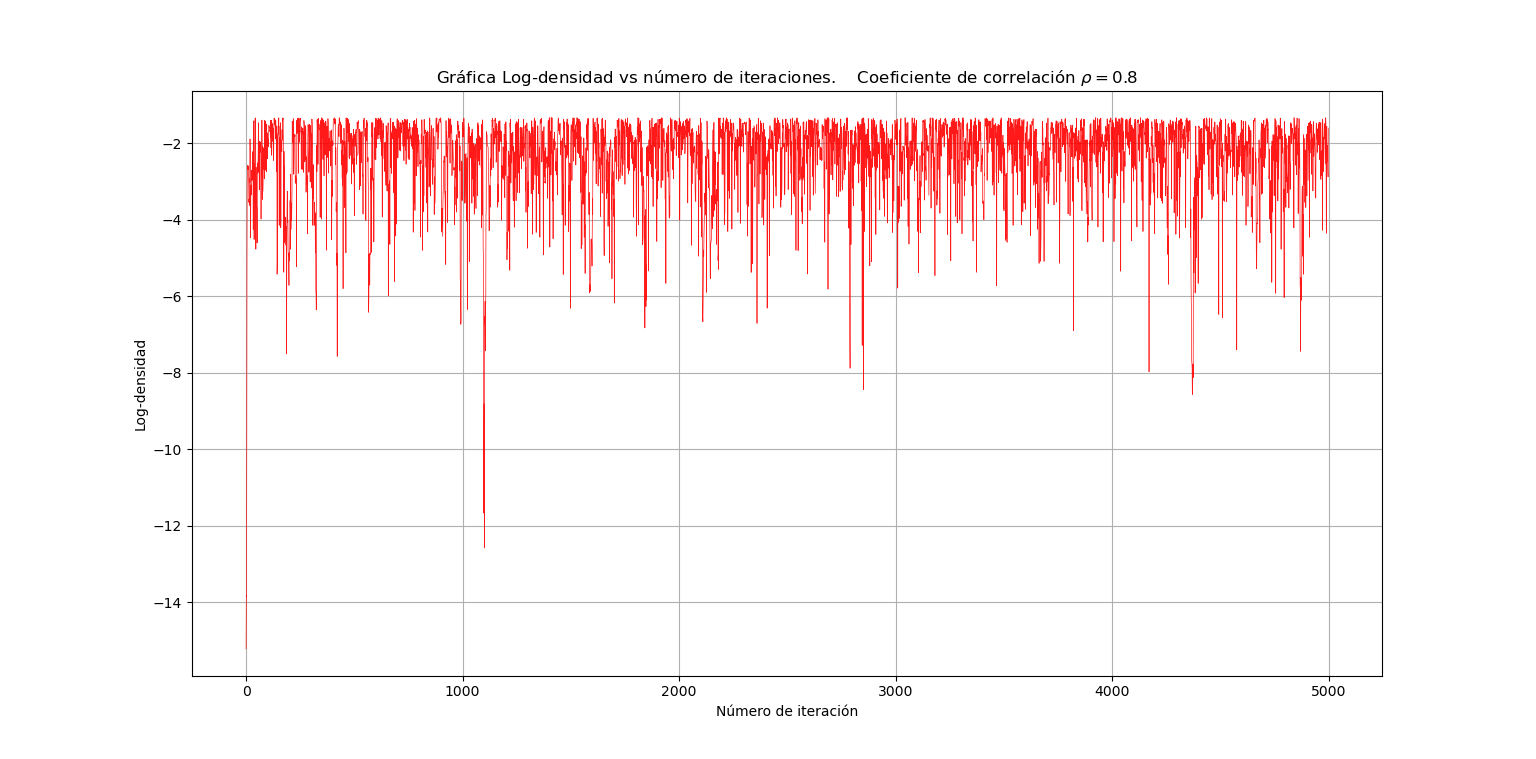
\includegraphics[width=\linewidth]{1.png}
        \caption{Log-densidad vs número de iteraciones. Coeficiente $\rho=0.8$}
    \end{figure} 
    Observamos que la gráfica de la log-densidad objetivo rápidamente llega a una sección que podemos intuir es estable. Esto nos hace tomar la decisión de 
    tomar un Burn-in igual a 250 iteraciones. Graficamos el recorrido de la cadena, el cual se aprecia en la figura 2.
    \begin{figure}[h!]
        \centering
        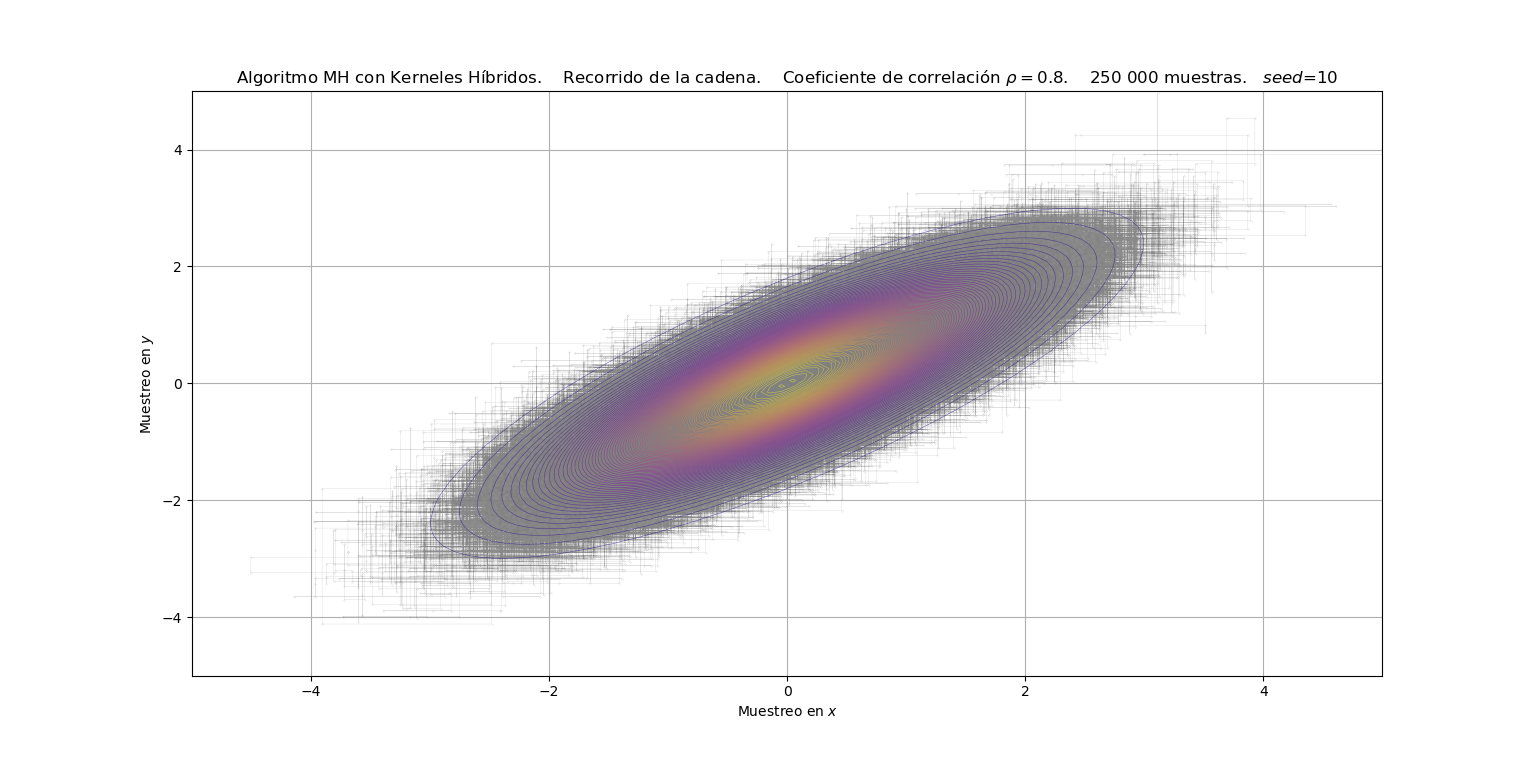
\includegraphics[width=\linewidth]{2.png}
        \caption{Recorrido de la cadena. Punto inicial $m=(5,5)$. Se puede apreciar una buena convergencia a la distribución objetivo.}
    \end{figure} 
    En esta figura observamos el comportamiento de los kerneles híbridos que actúan en solo una dirección: a cada iteración, de aceptar la 
    propuesta, se avanza o bien en la dirección horizontal o bien en la vertical. Observamos una rápida convergencia a la distribución objetivo, que en este caso
    es una normal bivariada, con matriz de covarianzas la dada al inicio de este ejercicio.  Graficamos ahora 
    los histogramas de la variable $x$ y la variable $y$. De acuerdo a la matriz de covarianzas,
    las variables marginales deben ser normales estándar.
    \begin{figure}[h!]
        \centering
        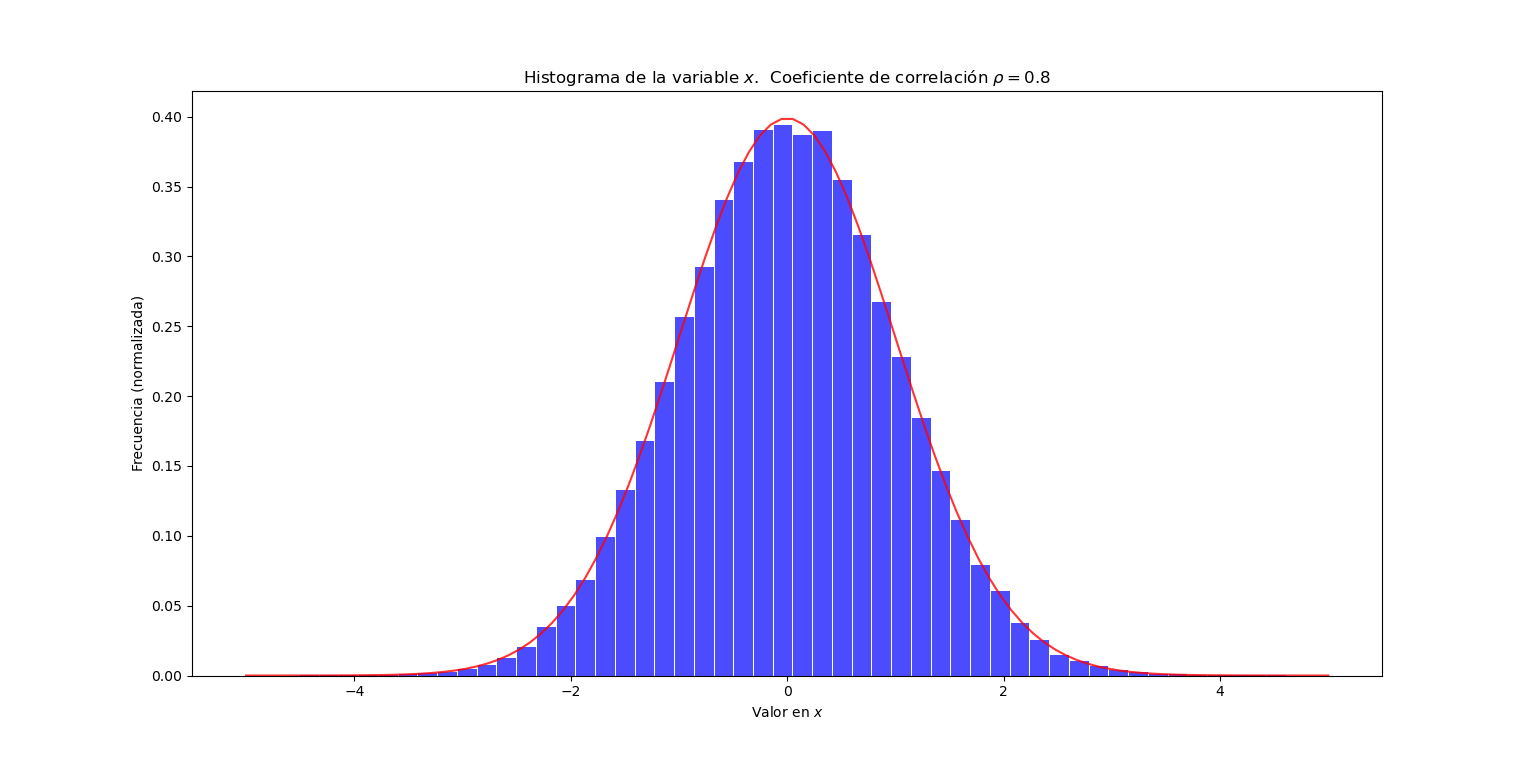
\includegraphics[width=\linewidth]{3.png}
        \caption{Histograma en $x$}
    \end{figure} 
    \begin{figure}[h!]
        \centering
        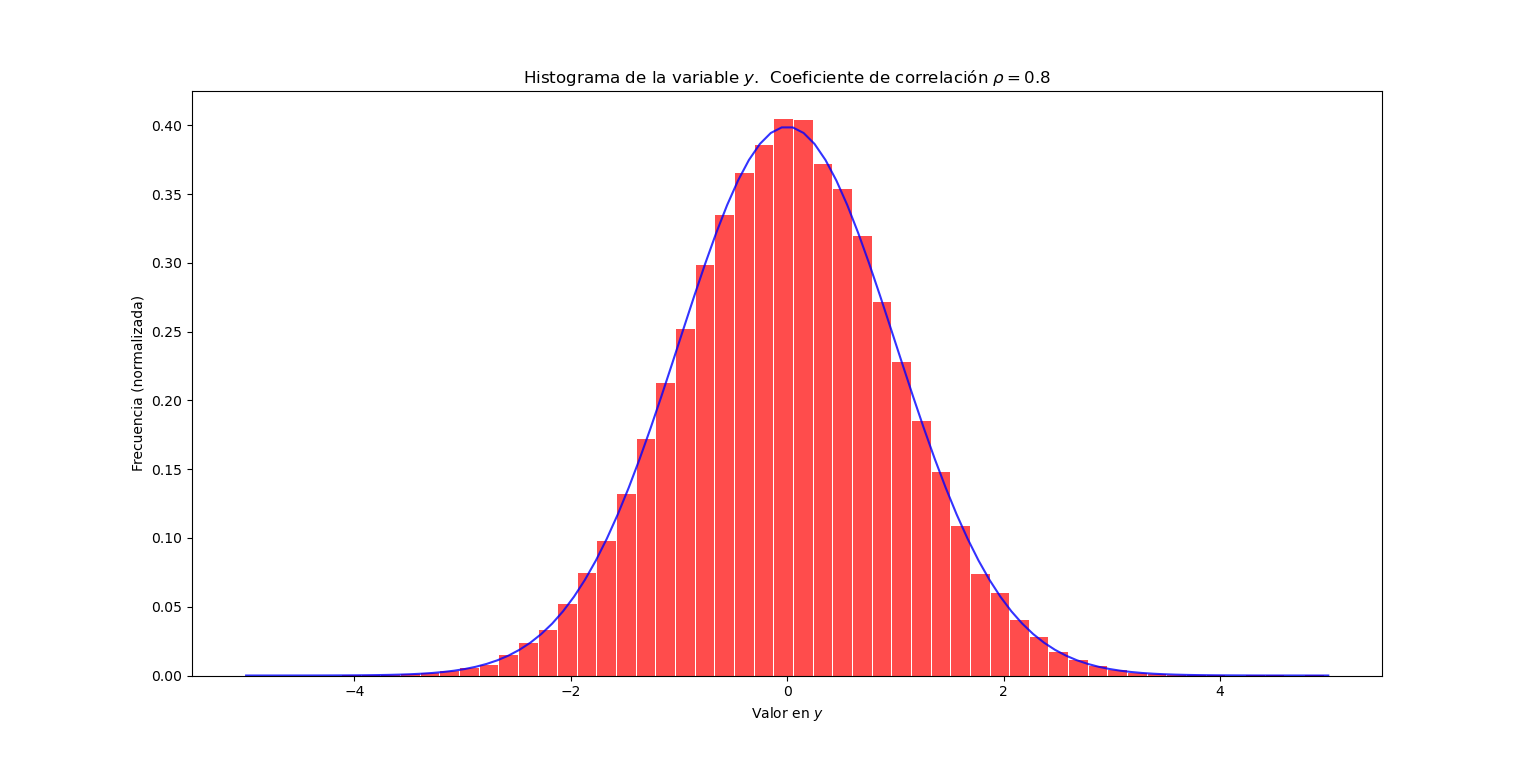
\includegraphics[width=\linewidth]{4.png}
        \caption{Histograma en $y$}
    \end{figure} 
    Las líneas dibujadas en ambos histogramas corresponden a las densidades de variables 
    aleatorias normales estándar. Esto comprueba lo mencionado anteriormente.\\
    
    Procedemos ahora con el ejemplo que utiliza $\rho=0.95$. Análogamente a lo hecho antes, se 
    obtienen los siguientes resultados:
    \begin{figure}[h!]
        \centering
        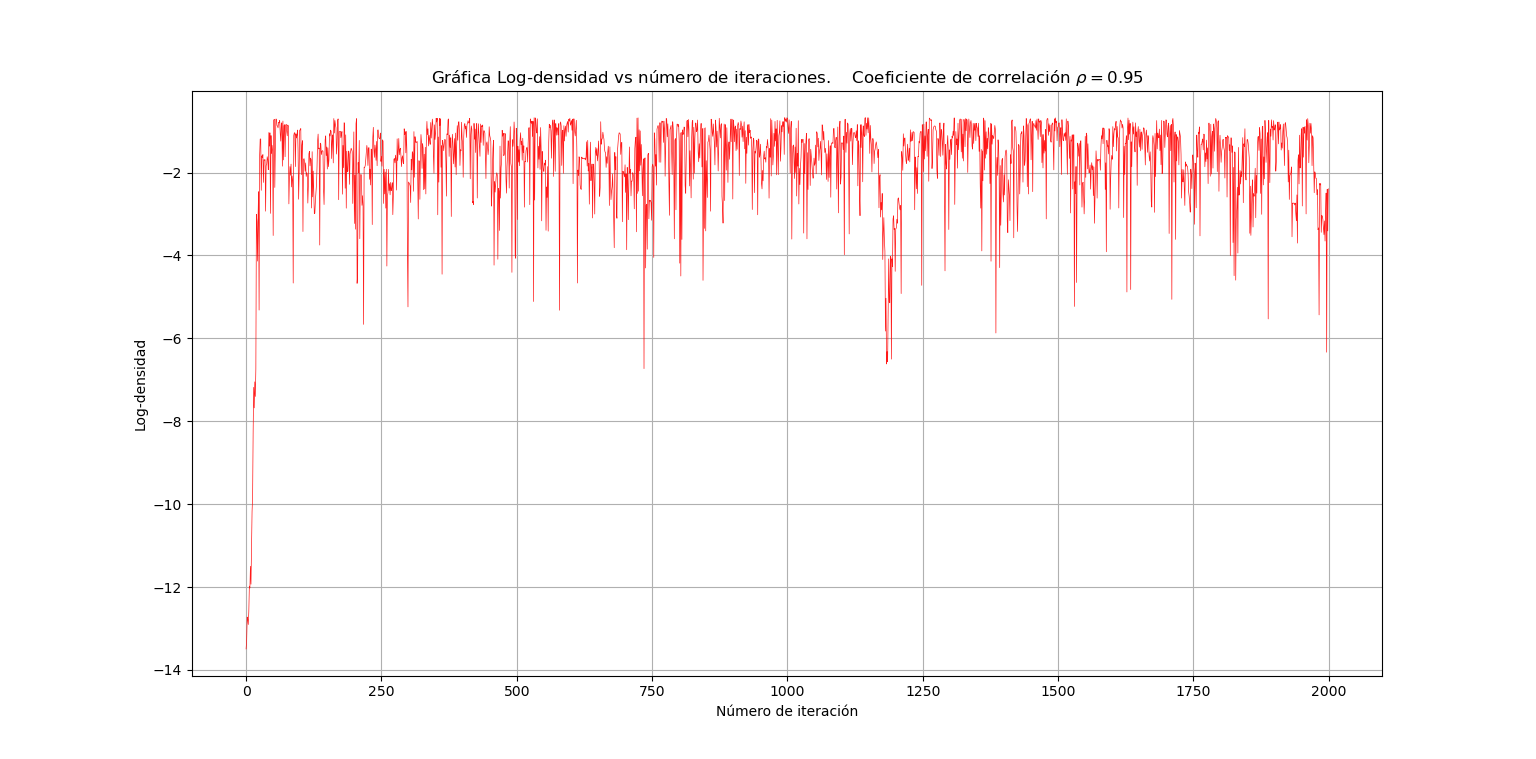
\includegraphics[width=\linewidth]{5.png}
        \caption{Log-densidad vs número de iteraciones. Caso $\rho=0.95$}
    \end{figure} 
    Tal y como en el primer caso, rápidamente la densidad llega a una zona de estabilidad. De la 
    visualización de la figura 5, deducimos que un Burn-in de tamaño 250 es 
    adecuado. Graficamos el recorrido de la cadena junto con las curvas de nivel 
    de la densidad objetivo. Esto se presenta en la figura 6.\\

    \begin{figure}[h!]
        \centering
        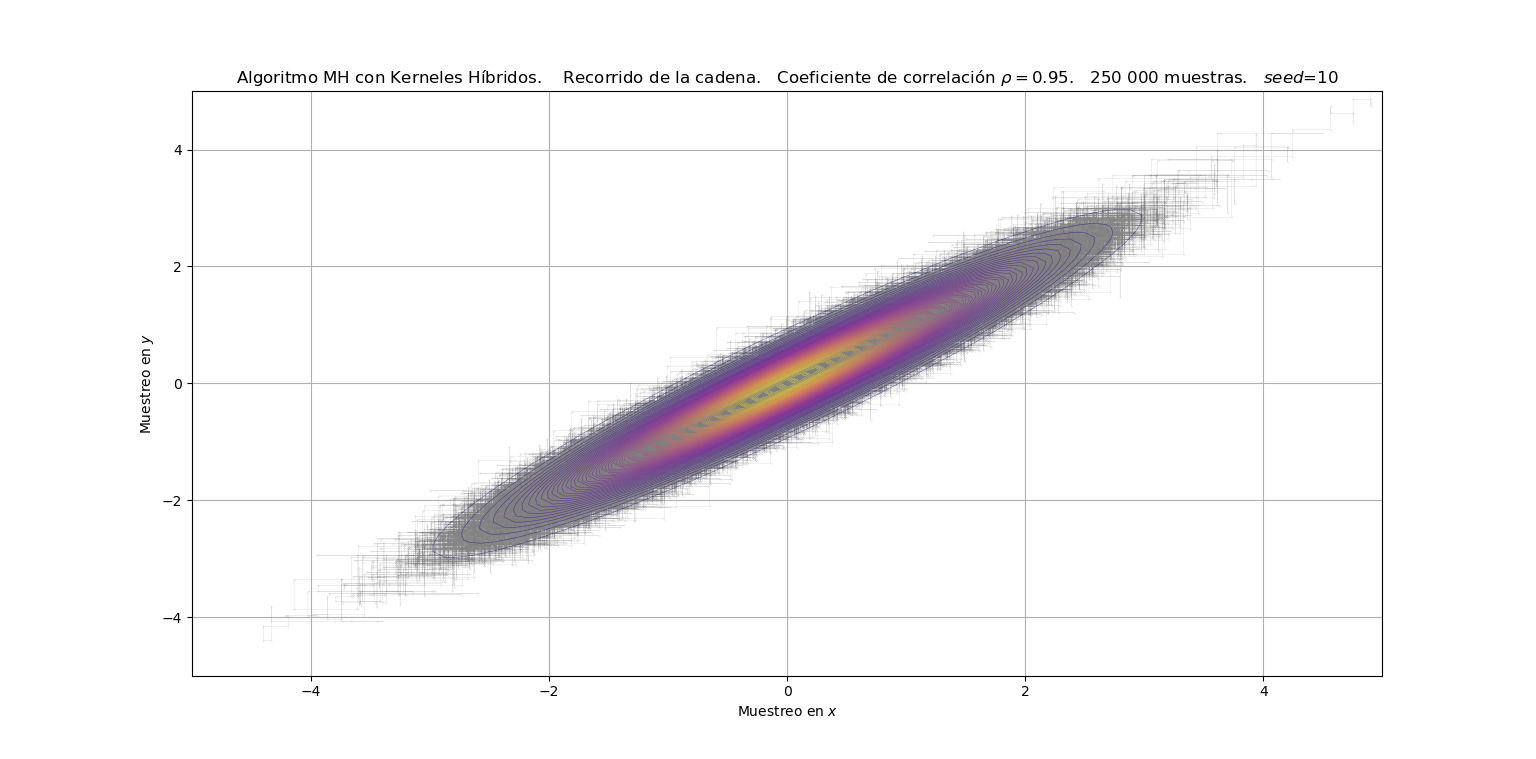
\includegraphics[width=\linewidth]{6.png}
        \caption{Recorrido de la cadena. Punto inicial $m=(5,5)$. De nuevo se visualiza una convergencia adecuada}
    \end{figure} 
    Presentamos también los histogramas de las variables $x$ y $y$. A pesar de 
    que el coeficiente de correlación ha cambiado (cosa que se refleja en la forma
    de la densidad conjunta en la figura 6) las marginales siguen siendo 
    variables normales estándar. Esto se puede comprobar con las figuras 7 y 8.\\

    \begin{figure}[h!]
        \centering
        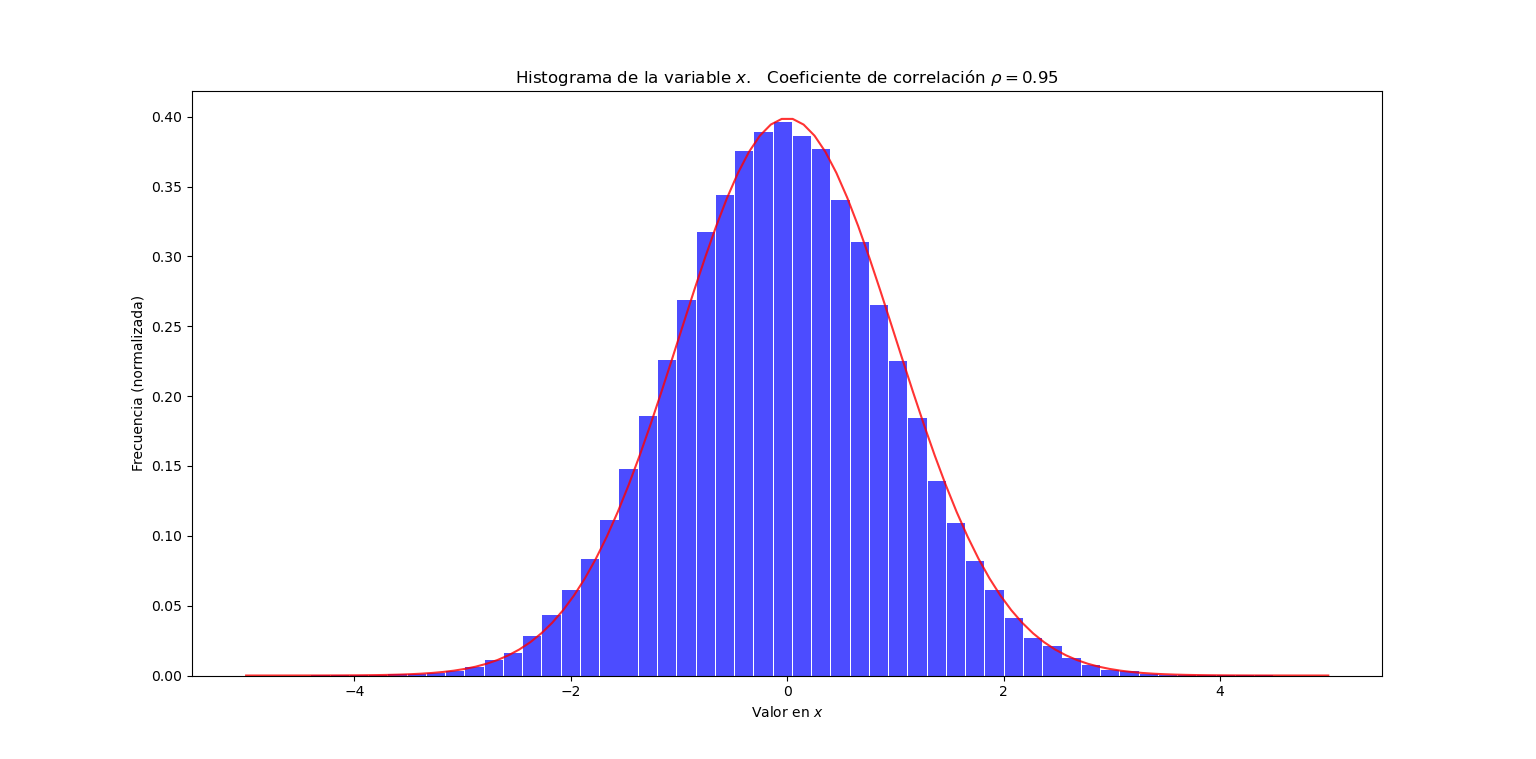
\includegraphics[width=\linewidth]{7.png}
        \caption{Histograma en $x$}
    \end{figure} 
    \begin{figure}[h!]
        \centering
        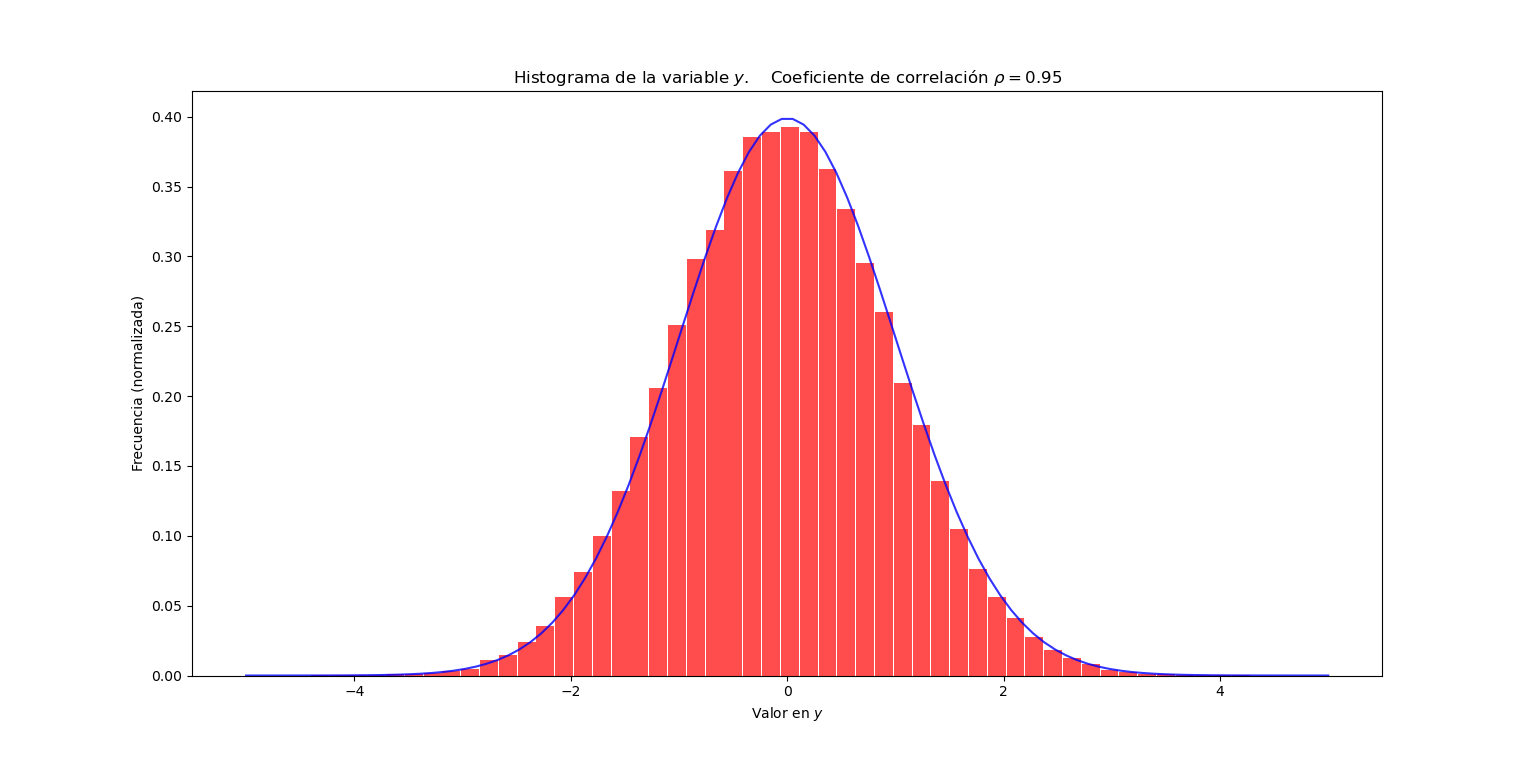
\includegraphics[width=\linewidth]{8.png}
        \caption{Histograma en $y$}
    \end{figure} 
    En estos histogramas nuevamente se dibuja la función de densidad de las variables 
    normales estándar. Tal y como se puede apreciar, estas encajan excelente con los 
    histogramas, tal y como era de esperarse.
    

    \item[\textbf{2.}] Considere los tiempos de falla $t_1,...,t_n$ con distribución $Weibull(\alpha,\lambda)$:
    \[
    f(t_i|\alpha,\lambda)=\alpha\lambda t_i^{\alpha-1}e^{-t^{-\alpha}_i\lambda}.   
    \]
    Se asumen como a priori $\alpha\sim\exp(c)$ y $\lambda|\alpha\sim \Gamma(\alpha,b)$, por lo tanto, 
    $f(\alpha,\lambda)=f(\lambda|\alpha)f(\alpha)$. Así, para la distribución posterior 
    se tiene: 
    \[
    f(\alpha,\lambda|\overline{t})\propto f(\overline{t}|\alpha,\lambda)f(\alpha,\lambda).    
    \]
    A partir del algoritmo MH usando Kerneles híbridos simule valores de la distribución posterior 
    $f(\alpha,\lambda|\overline{t})$, considerando las siguientes propuestas:\\

    \underline{Propuesta 1}:
    \[
    \lambda_p|\alpha,\overline{t}\sim Gamma \left(\alpha+n,b+\sum_{i=1}^{n}t_i^{\alpha}\right)    
    \]
    y dejando $\alpha$ fijo.\\

    \underline{Propuesta 2:}
    \[
        \alpha_p|\lambda,\overline{t}\sim Gamma(n+1,-\log(b)-\log(r_1)+c),  
    \]
    con $r_1=\prod_{i=1}^{n}t_i$. y dejando $\lambda$ fijo.\\

    \underline{Propuesta 3:} 
    \[
    \alpha_p\sim \exp(c) \text{ y } \lambda_p|\alpha_p \sim Gamma(\alpha_p,b).    
    \]

    \underline{Propuesta 4 (RWMH):}
    \[
    \alpha_p=\alpha+\varepsilon,    
    \]
    con $\varepsilon\sim N(0,\sigma)$ y dejando $\lambda$ fijo. 

    Simular datos usando $\alpha=1$ y $\lambda=1$ con $n=20$. Para la a priori usar $c=1$ y $b=1$.\\

    \textbf{Solución:} Implementamos el algoritmo de Metrópolis Hastings utilizando Kérnel Híbrido y Gibbs sampler. Observamos que 
    en este caso tenemos 4 propuestas para realizar la implementación. En clase se argumentó que la primera de ellas, la cual consiste en
    muestrear el valor de $\lambda_p|\alpha$ es un Gibbs Sampler, por lo que la probabilidad de aceptar dicha propuesta siempre es 1.
    No obstante, las demás propuestas no necesariamente cumplen con esto, ya que por ejemplo la propuesta 4 consiste en un Random Walk Metrópolis Hastings.\\

    Para implementar el algoritmo se coloca primero la semilla $seed=20$ para replicar resultados. Posteriormente se crean las funciones que recrean la distribución objetivo 
    y cada una de las cuatro propuestas que se mencionan en este problema. En particular, la función de la propuesta número 4 es tal que utiliza una variable aleatoria 
    $Normal(0,0.25)$ para implementar el RWMH de dicha propuesta. 
    \newline

    Se crea también la función que ejecutará el algoritmo de Metrópolis. Se otorga un peso igual a 1/4 a cada uno de las cuatro propuestas, utilizando para ello
    una variable uniforme en $[0,1]$ y ejecutando una de las cuatro propuestas dependiendo de si la variable uniforme cayó en alguno de los 4 subintervalos del $[0,1]$ 
    correspondiente a cada variable. A saber, la propuesta 1 correspondía a un valor de una uniforme en [0,0.25], la propuesta 2 correspondía a un 
    valor de la uniforme en [0.25,0.5], etc.
    \newline

    Se simulan los datos de la distribución $Weibull(1,1)$ utilizando $scipy$, y se selecciona como punto inicial al punto $m=(2,2)$.
    Se fija un número de iteraciones $k=250,000$. Se obtienen los siguientes
    resultados gráficos: comenzando con la log-densidad objetivo para obtener el Burn-in, se obtiene el contenido de la figura 9.\\
    \begin{figure}[h!]
        \centering
        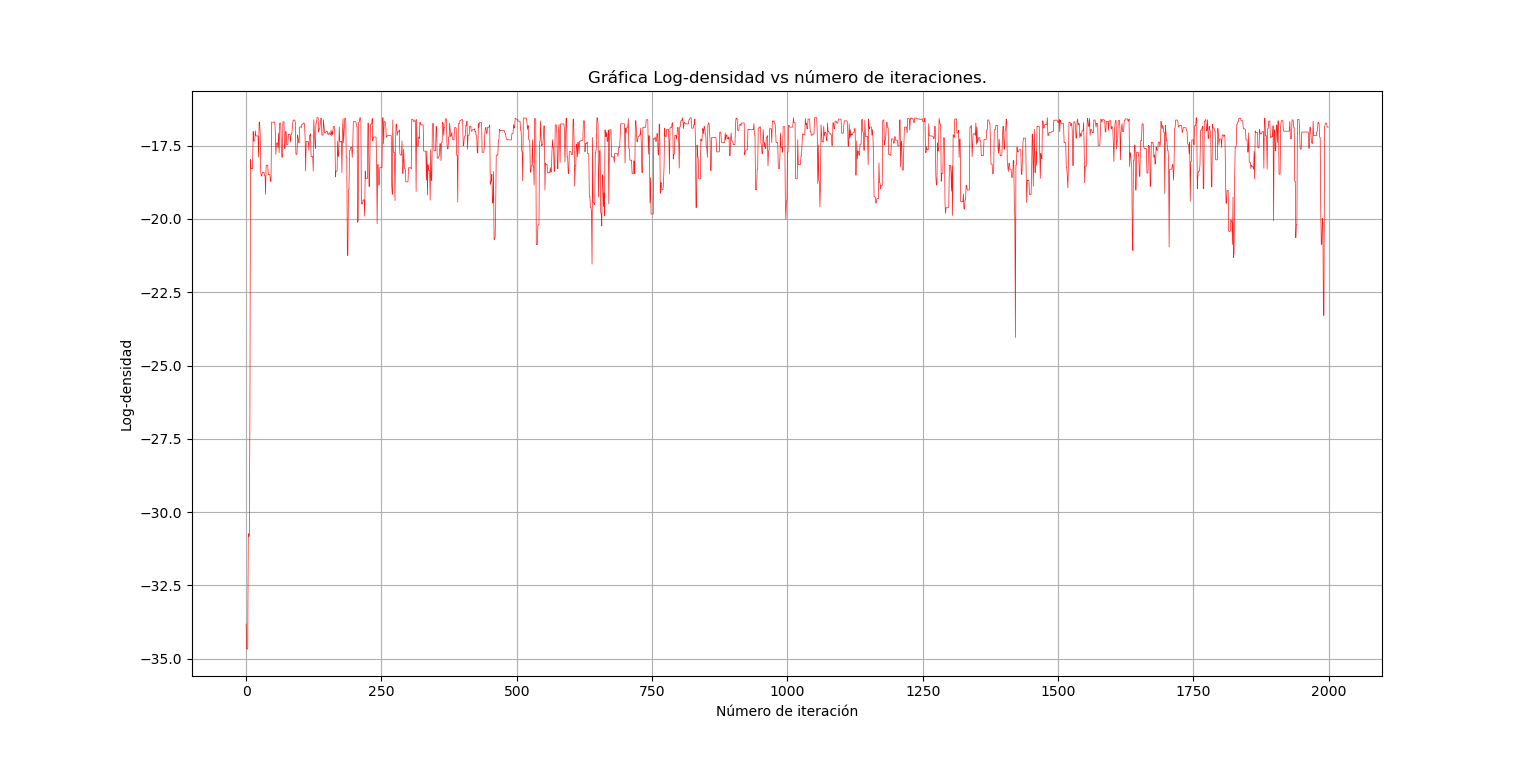
\includegraphics[width=\linewidth]{9.png}
        \caption{Log-densidad vs número de iteraciones en el ejercicio 2.}
    \end{figure} 
    Nuevamente del comportamiento de esta gráfica concluimos que un valor de Burn-in igual a 250 es adecuado. Se imprime ahora la gráfica del recorrido de la cadena, obteniendo 
    el resultado de la figura 10.\\
    \begin{figure}[h!]
        \centering
        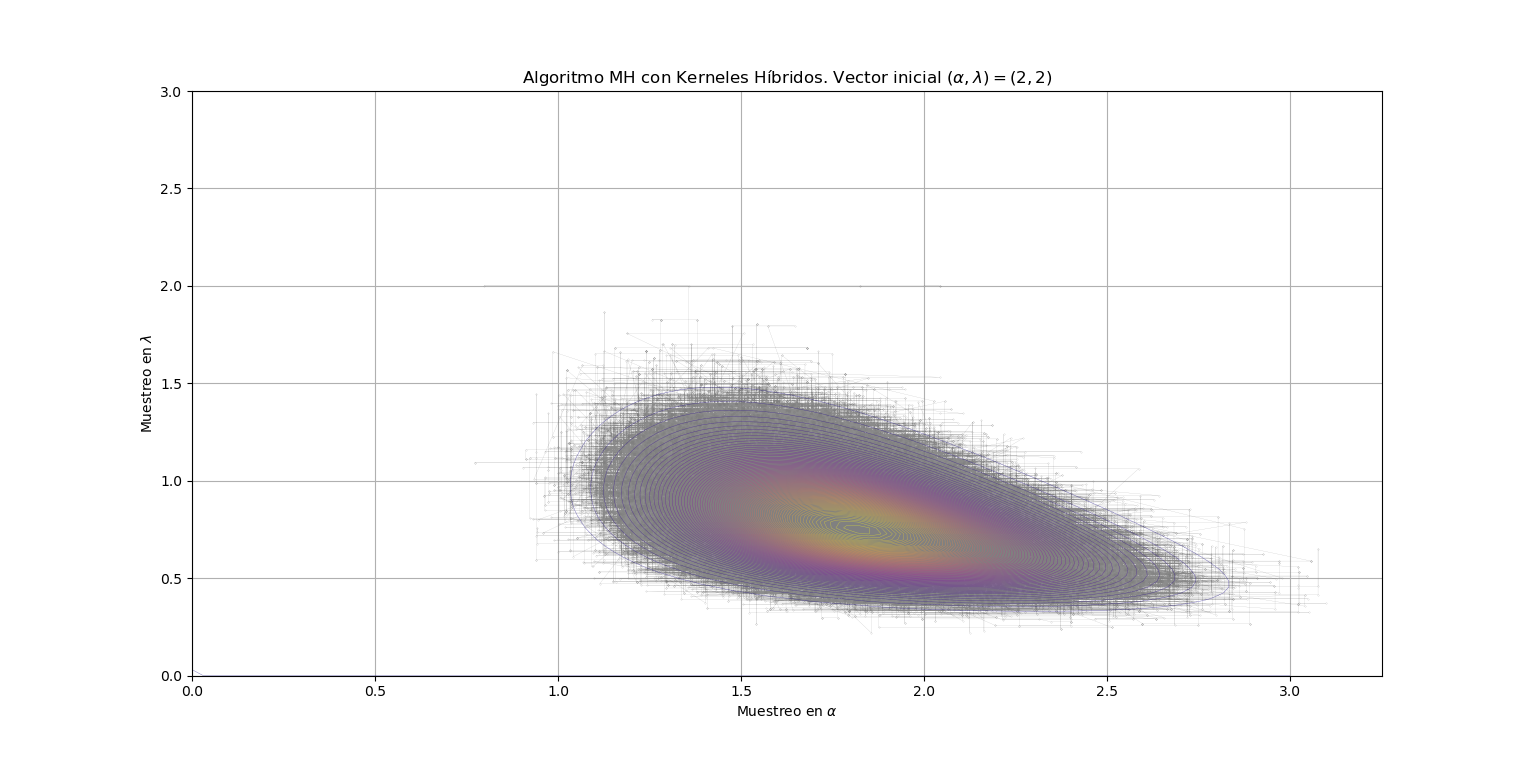
\includegraphics[width=\linewidth]{10.png}
        \caption{Recorrido de la cadena y curvas de nivel de la distribución objetivo. Observamos un buen desempeño.}
    \end{figure} 
    De la figura se puede observar un buen comportamiento de la cadena en cuanto a su aproximación a la distribución objetivo. Para visualizar el comportamiento 
    más de cerca de las variables $\lambda$ y $\alpha$, imprimimos el histograma de cada una de estas variables. Esto se presenta en las figuras 11 y 12.
    \begin{figure}[h!]
        \centering
        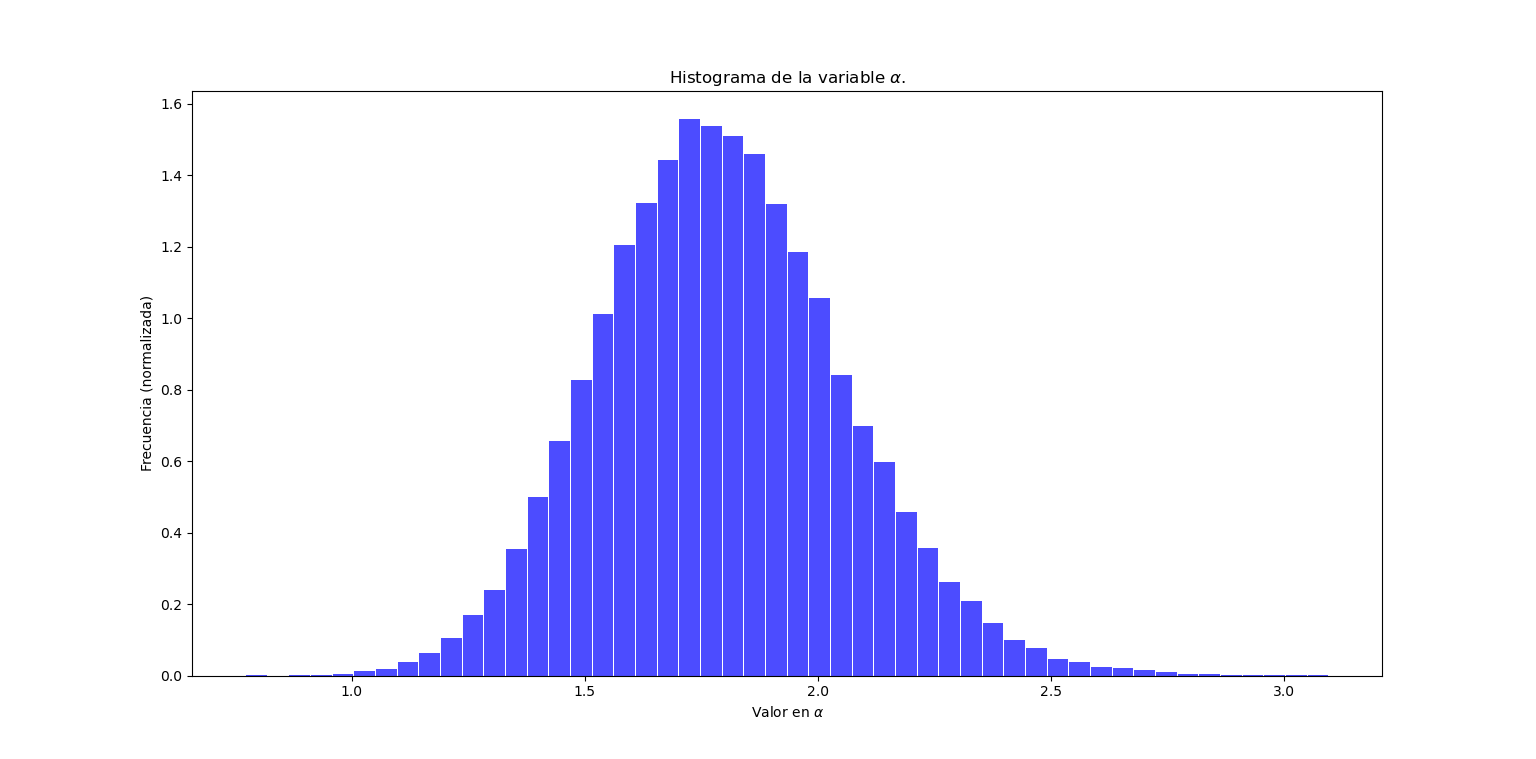
\includegraphics[width=\linewidth]{11.png}
        \caption{Histograma de la variable $\alpha$}
    \end{figure} 
    \begin{figure}[h!]
        \centering
        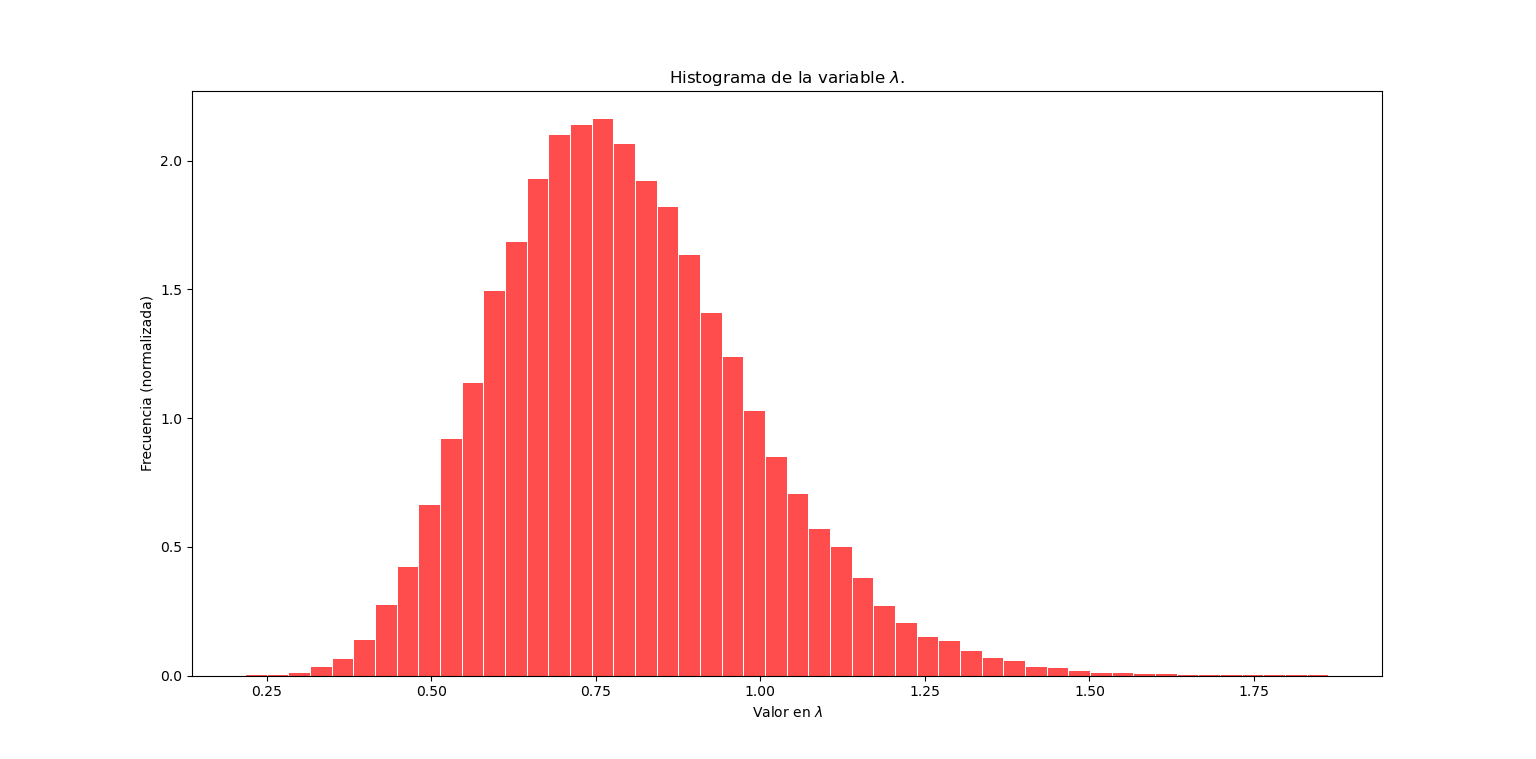
\includegraphics[width=\linewidth]{12.png}
        \caption{Histograma de la variable $\lambda$}
    \end{figure} 
    Observamos un comportamiento en la variable $\alpha$ que tiene una media de aproximadamente $1.7$, mientras 
    que en la variable $\lambda$ se observa una media de aproximadamente $0.7$. 



    \item[\textbf{3.}] Considere el ejemplo referente al número de fallas de bombas de agua en una 
    central nuclear, donde $p_i$ representa el número de fallas en el tiempo de operación $t_i$, con $i=1,...,10$.\\

    Se considera el modelo $p_i\sim Poisson(\lambda_it_i)$, (las $\lambda_i$ son independientes entre sí), con 
    distribuciones a priori $\lambda_i|\beta \sim Gamma(\alpha,\beta)$ y $\beta\sim Gamma(\gamma, \delta)$, por lo tanto:
    \[
    f(\lambda_1,...,\lambda_n,\beta)=f(\lambda_1|\beta)f(\lambda_2|\beta)\cdot...\cdot f(\lambda_n|\beta)f(\beta).    
    \]
    Para la distribución posterior se tiene:
    \[
    f(\lambda_1,...,\lambda_n,\beta|\overline{p})\propto L(\overline{p},\overline{\lambda},\beta)f(\lambda_1,...,\lambda_n,\beta).    
    \]
    Simule valores de la distribución posterior $f(\lambda_1,...,\lambda_n,\beta|\overline{p})$, usando un 
    kernel híbrido, considerando las propuestas:
    \[
    \lambda_i|\overline{\lambda}_{-i},\beta,\overline{t} \sim Gamma(p_i+\alpha,\beta+t_i).    
    \]
    \begin{table}[]
        \begin{tabular}{|l|l|l|l|l|l|l|l|l|l|l|}
        \hline
        Bomba ($i$)          & 1     & 2     & 3     & 4      & 5    & 6     & 7    & 8    & 9   & 10    \\ \hline
        T. de uso $t_i$      & 94.32 & 15.72 & 62.88 & 125.76 & 5.24 & 31.44 & 1.05 & 1.05 & 2.1 & 10.48 \\
        \# de fallas $(p_i)$ & 5     & 1     & 5     & 14     & 3    & 17    & 1    & 1    & 4   & 22    \\ \hline
        \end{tabular}
        \caption{Datos de bombas de agua en centrales nucleares (Robert y Casella, p.385) par ael ejemplo 8.3.}
    \end{table}
    \[
    \beta|\overline{\lambda},\overline{t}\sim Gamma\left(n\alpha+\gamma,\delta+\sum_{i=1}^{n}\lambda_i\right).
    \]
    Verifique que estas son propuestas Gibbs.

    Use los datos de la tabla 1 con los parámetros a priori $\alpha=1.8$, $\gamma=0.01$ y $\delta=1$.\\

    \textbf{Solución:} para este último ejercicio, primero se fija la semilla en el valor $seed=10$ para replicar resultados. Posteriormente, 
    se definen las funciones a utilizar. En este caso, y dada la particularidad de las propuestas a usar, para implementar
    el algoritmo no es necesario hallar explícitamente la distribución objetivo, ya que las propuestas 
    se componen de Kerneles Gibbs, por lo que el cociente de Metrópolis-Hastings será siempre 1 
    y con ello las propuestas hechas siempre serán aceptadas. El que los Kérneles presentados tengan 
    esta propiedad se muestra al final de los resultados de este ejercicio.
    \newline

    Se define el vector inicial $m=(5,5,...,5)=(\lambda_1,\lambda_2,...,\lambda_{10},\beta)$, y se definen 
    dos funciones para ejecutar las propuestas. La primera de ellas consiste en realidad en una anidación de 
    las propuestas para los 10 parámetros $\lambda_1,...,\lambda_{10}$.\\

    Dicha función denominada $propuesta1$ consiste en simular variables $gamma$ dependiendo 
    del parámetro $i$ que sea ingresado, y que corresponde al valor de $\lambda_i$ en cuestión.
    \newline

    La segunda función $propuesta2$ consiste en simular valores para el parámetro $\beta$ a partir de 
    los datos que se tienen sobre $\lambda_1,...,\lambda_{10}$ y los datos.
    \newline

    Se crea la función $MH\_gibbs3$ que implementará el algoritmo. Dicha función crea una 
    variable uniforme. Se divide el intervalo [0,1] en 11 pedazos, y si la variable uniforme 
    cae en el último de los 11 pedazos, se procede a actualizar el parámetro $\beta$ de acuerdo 
    a la propuesta 2, mientras que si cae en los primeros 11 pedazos, se utiliza nuevamente 
    una variable aleatoria uniforme, pero esta vez discreta en el conjunto $\{1,...,10\}$ para 
    seleccionar el parámetro $\lambda_{i}$ que será actualizado. Lo anterior asegura que los kérneles que se seleccionan 
    tienen todos ellos igual peso entre sí.
    \newline

    Se cargan los datos del cuadro 1, y fijando $k=250,000$ iteraciones, se procede a la ejecución del algoritmo.
    De manera completamente heurística, y a falta del cálculo de la distribución objetivo de manera explícita, 
    se utiliza un Burn-in de tamaño 250 siendo congruente con lo visto en los otros ejercicios de esta tarea y de tareas 
    pasadas.\\

    Con tal Burn-in, se obtienen los histogramas de cada uno de los 11 parámetros $\lambda_1,...,\lambda_{10},\beta$, 
    los cuales son presentados en las figuras 13 en adelante. 
    \newline
    \begin{figure}[h!]
        \centering
        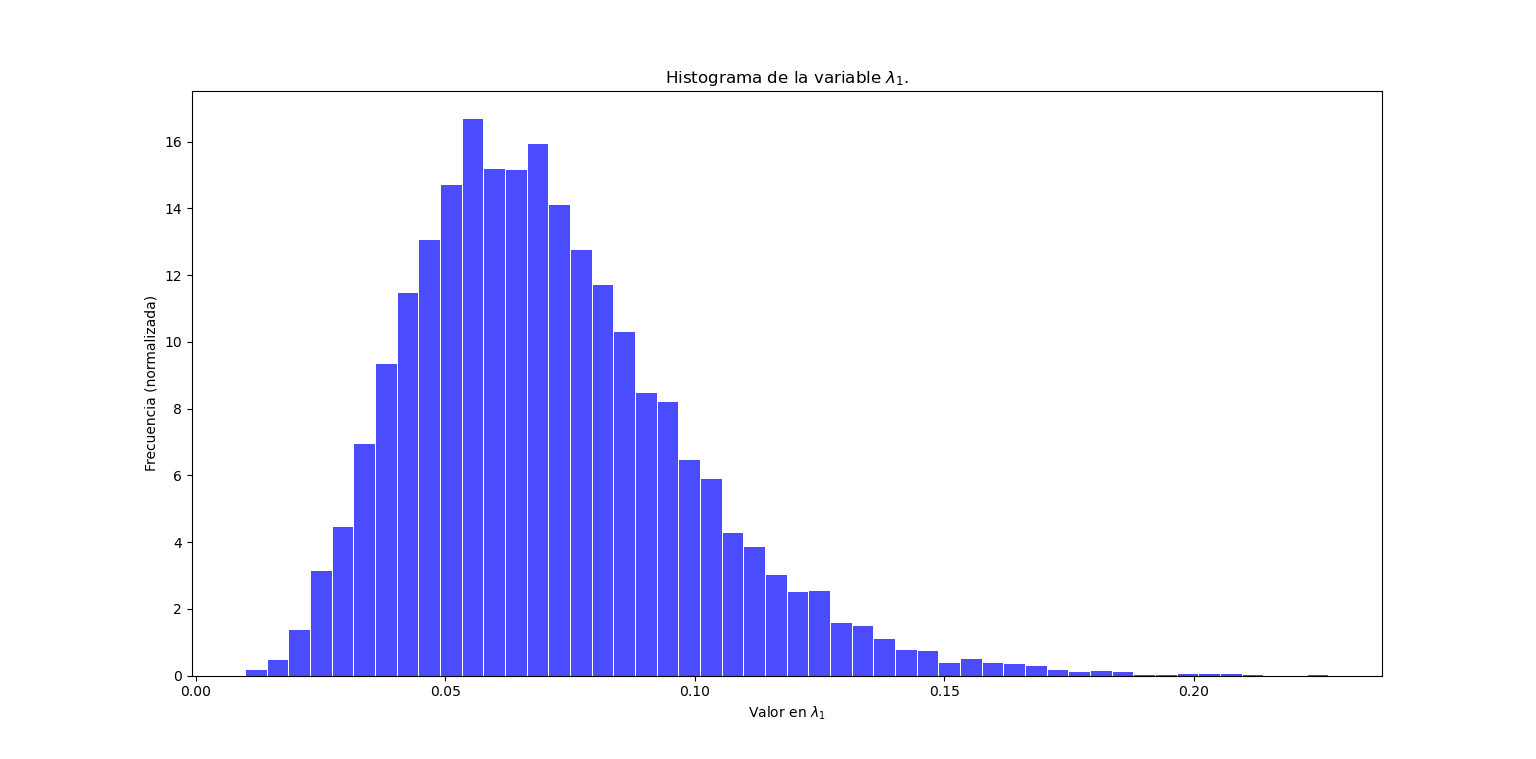
\includegraphics[width=\linewidth]{13.png}
        \caption{Histograma para $\lambda_{1}$}
    \end{figure} 
    \begin{figure}[h!]
        \centering
        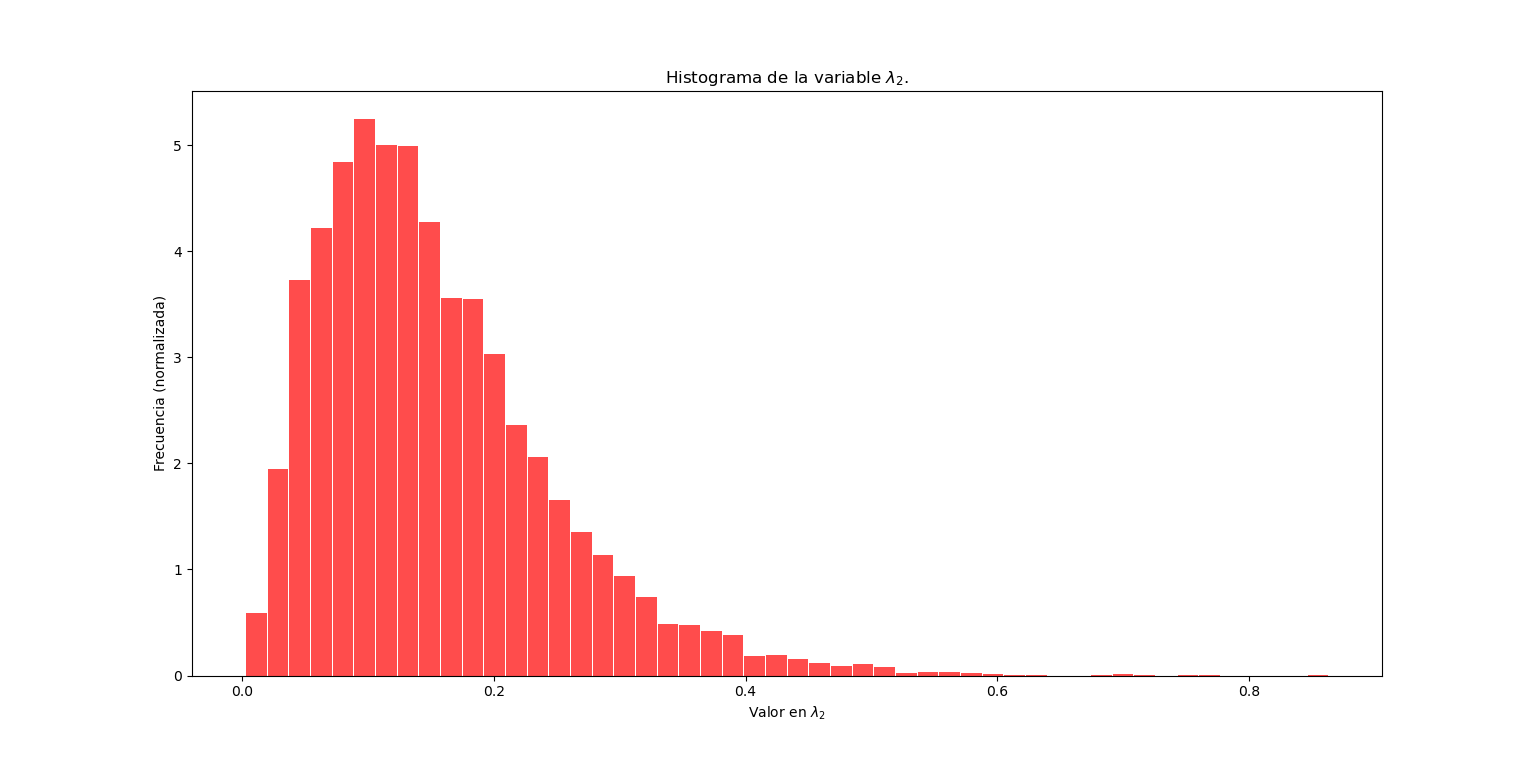
\includegraphics[width=\linewidth]{14.png}
        \caption{Histograma para $\lambda_{2}$}
    \end{figure} 
    \begin{figure}[h!]
        \centering
        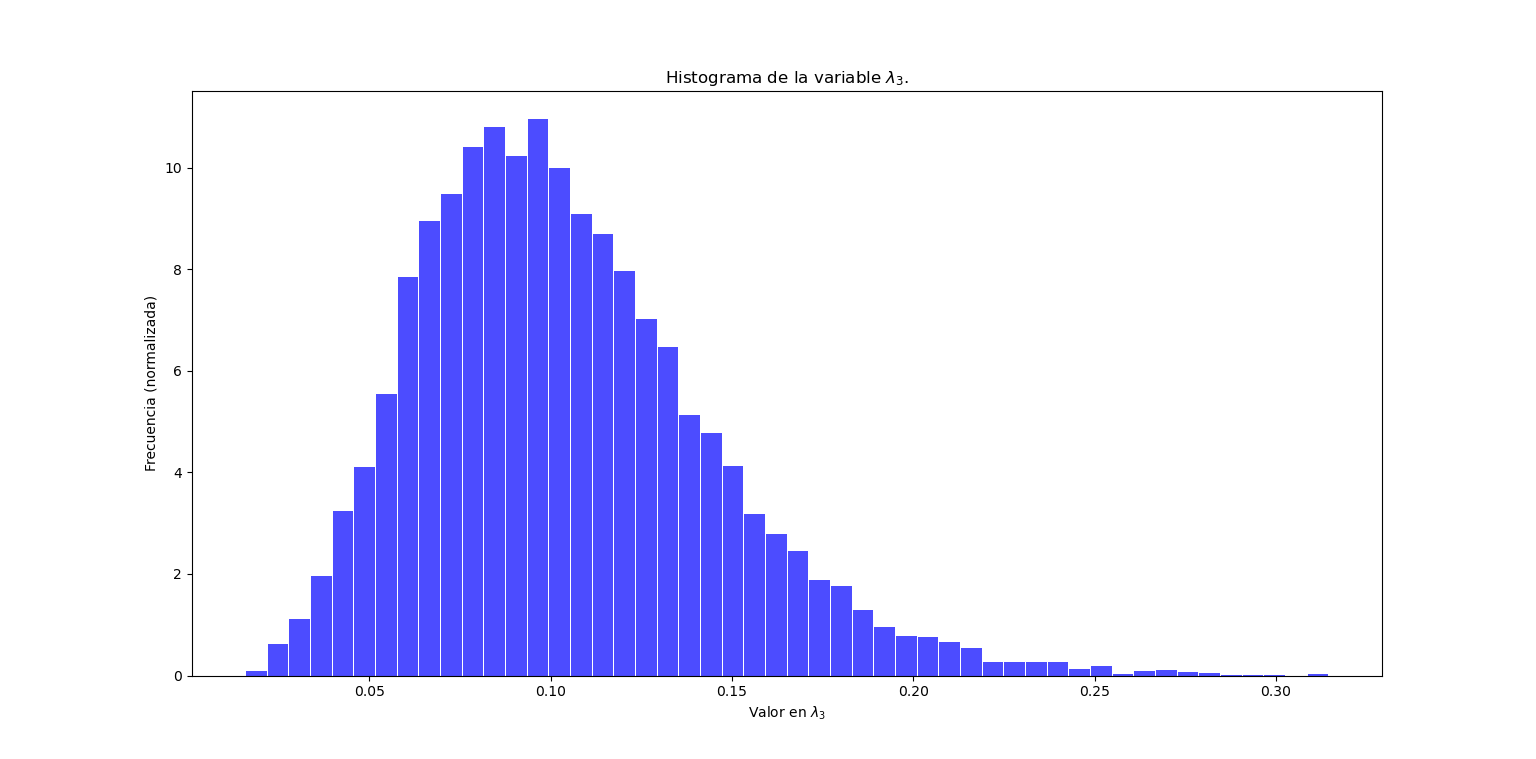
\includegraphics[width=\linewidth]{15.png}
        \caption{Histograma para $\lambda_{3}$}
    \end{figure} 
    \begin{figure}[h!]
        \centering
        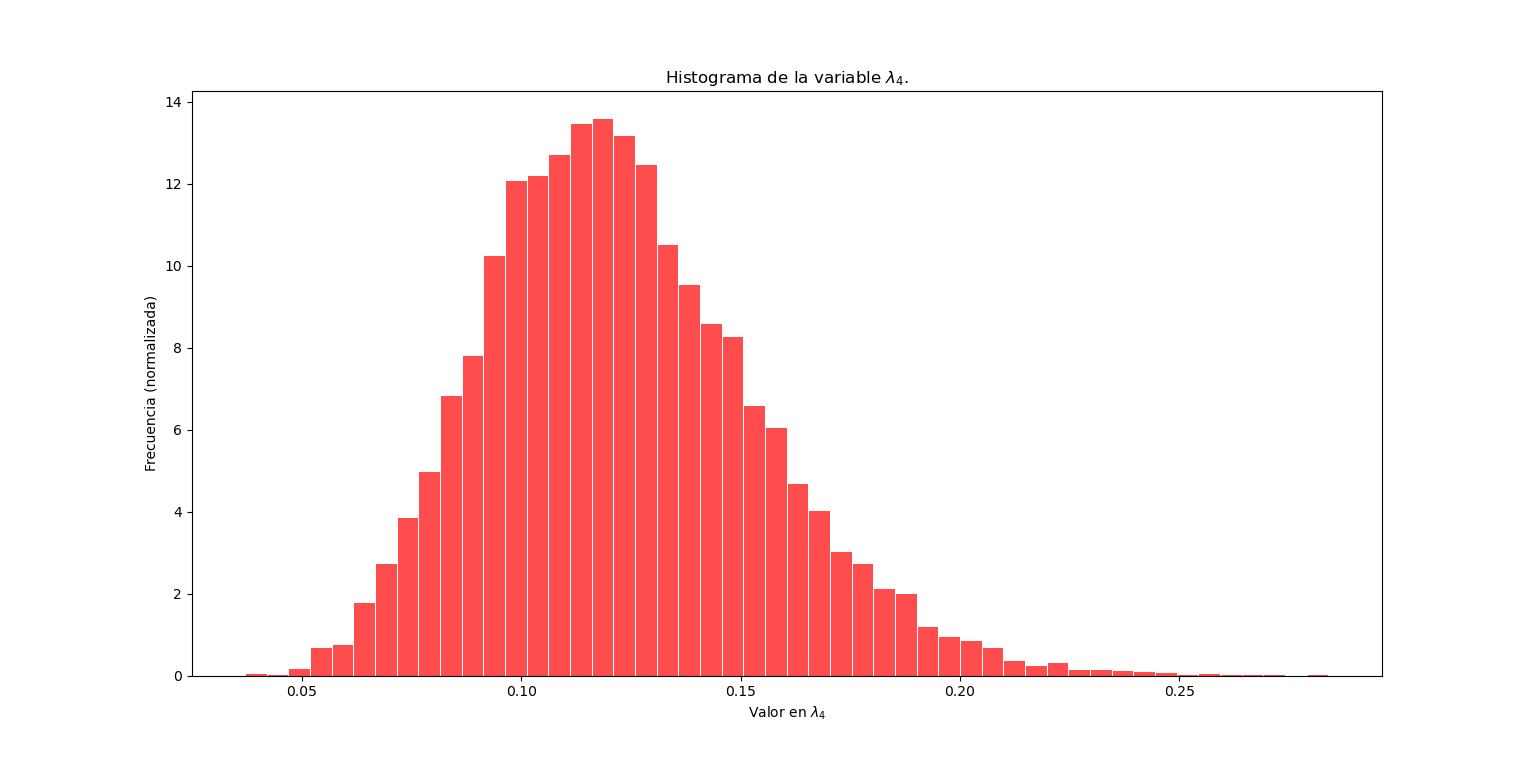
\includegraphics[width=\linewidth]{16.png}
        \caption{Histograma para $\lambda_{4}$}
    \end{figure} 
    \begin{figure}[h!]
        \centering
        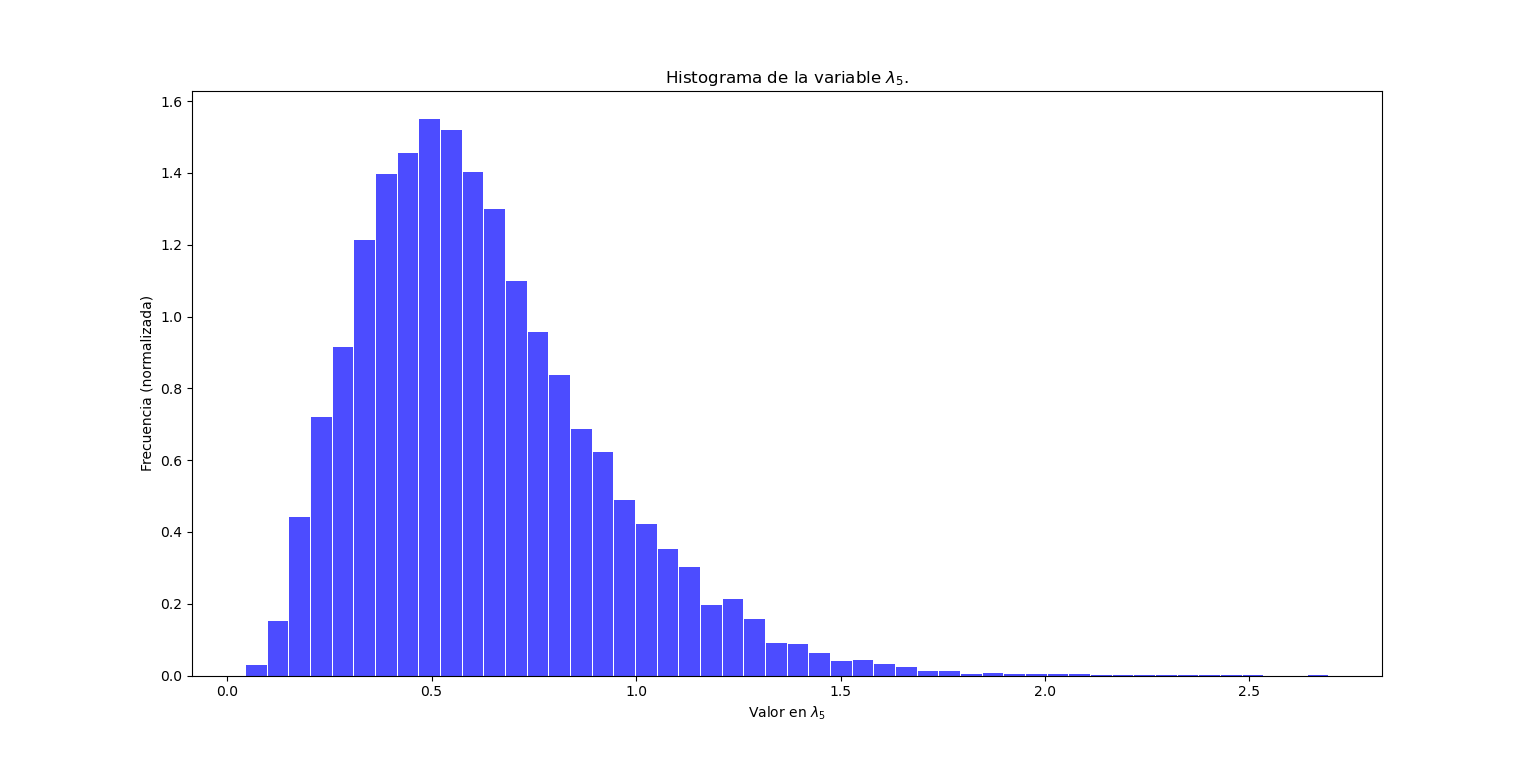
\includegraphics[width=\linewidth]{17.png}
        \caption{Histograma para $\lambda_{5}$}
    \end{figure} 
    \begin{figure}[h!]
        \centering
        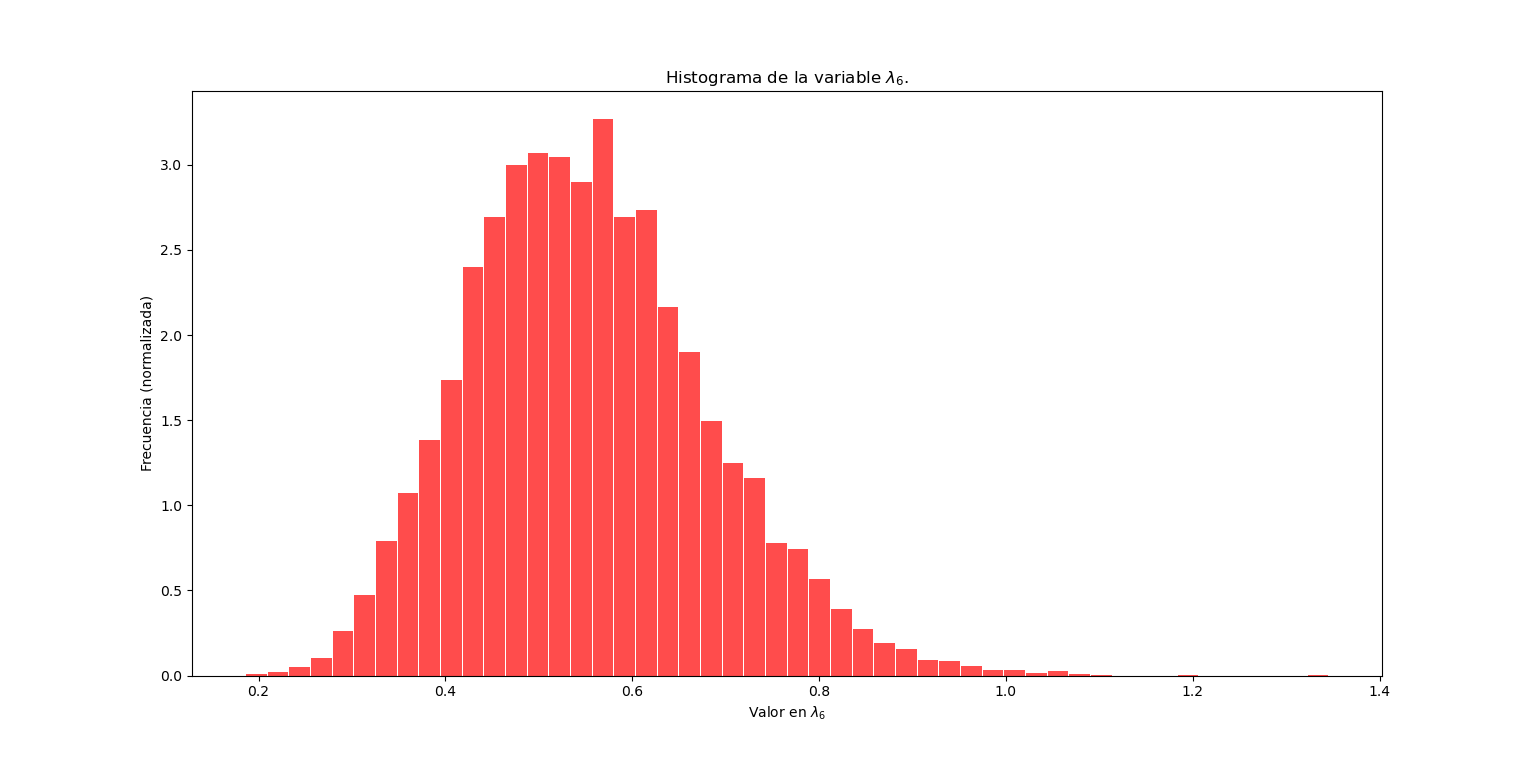
\includegraphics[width=\linewidth]{18.png}
        \caption{Histograma para $\lambda_{6}$}
    \end{figure} 
    \begin{figure}[h!]
        \centering
        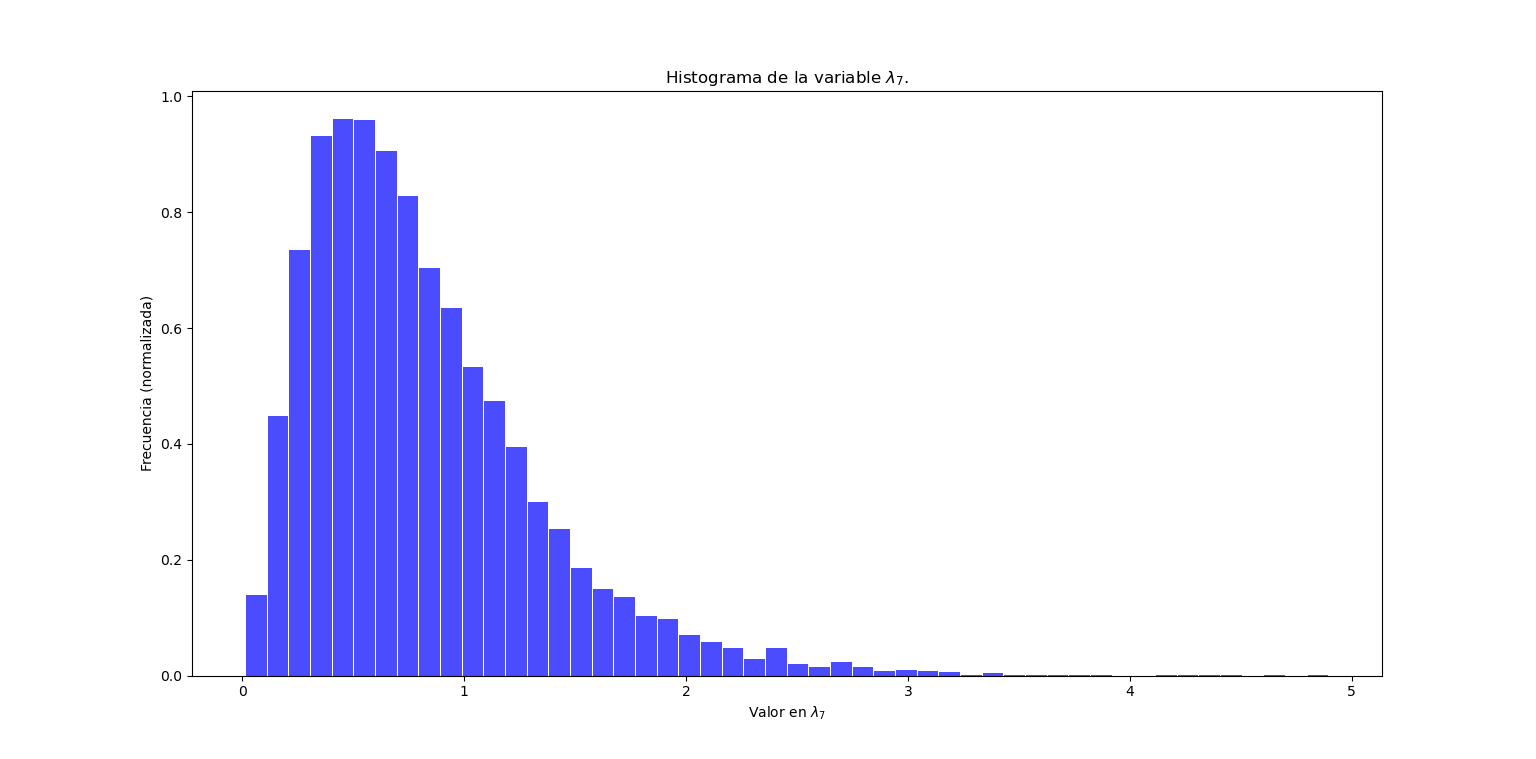
\includegraphics[width=\linewidth]{19.png}
        \caption{Histograma para $\lambda_{7}$}
    \end{figure} 
    \begin{figure}[h!]
        \centering
        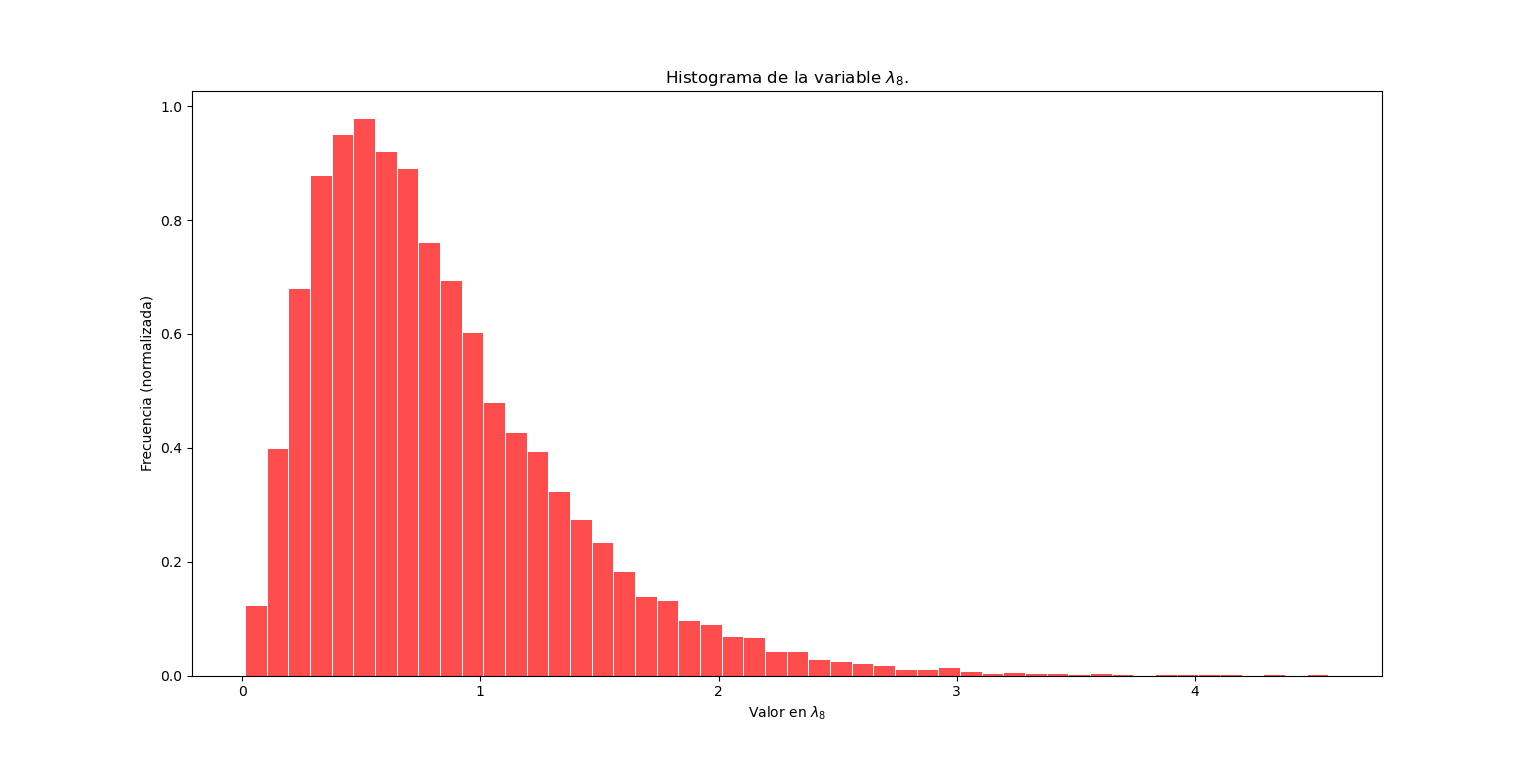
\includegraphics[width=\linewidth]{20.png}
        \caption{Histograma para $\lambda_{8}$}
    \end{figure} 
    \begin{figure}[h!]
        \centering
        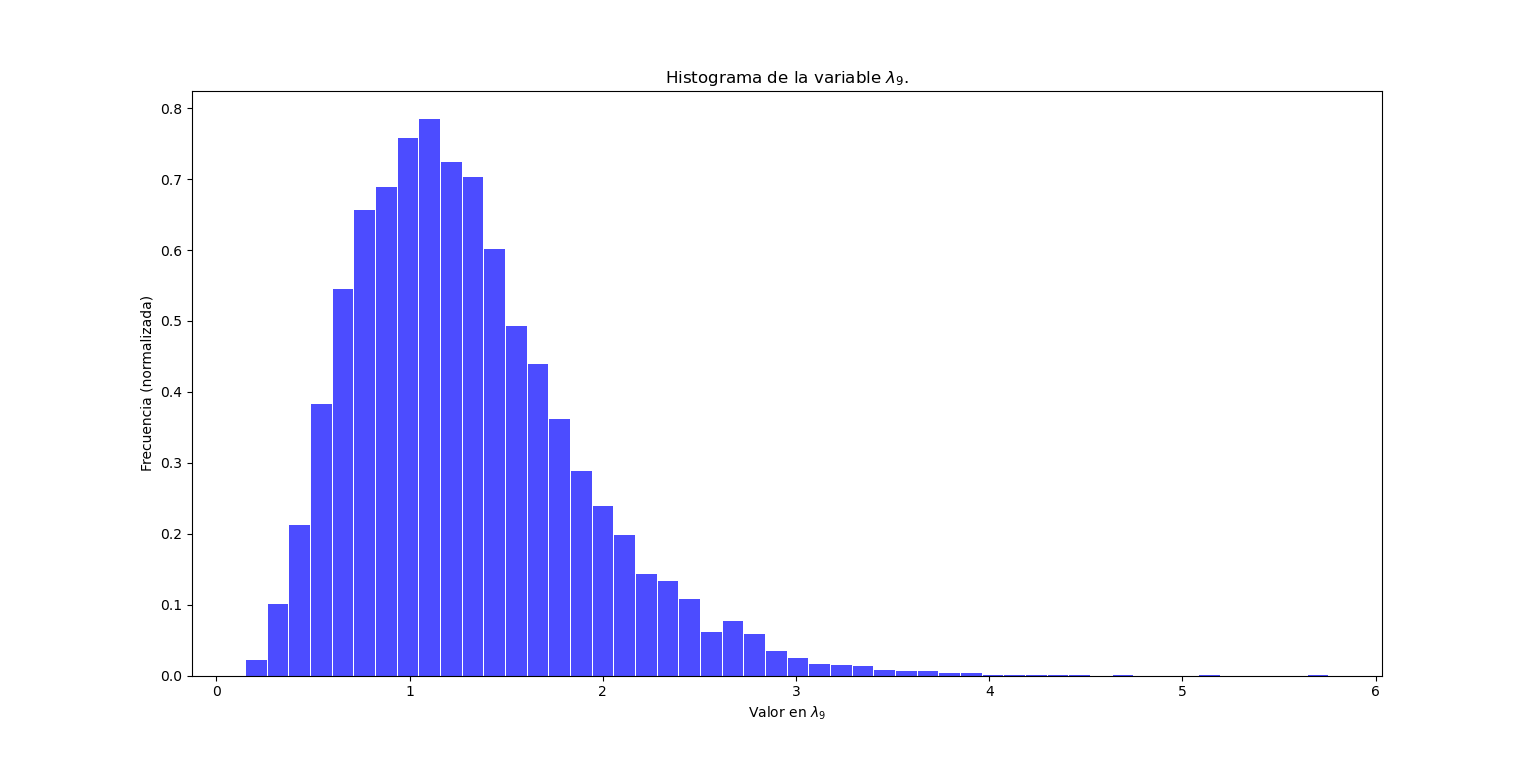
\includegraphics[width=\linewidth]{21.png}
        \caption{Histograma para $\lambda_{9}$}
    \end{figure} 
    \begin{figure}[h!]
        \centering
        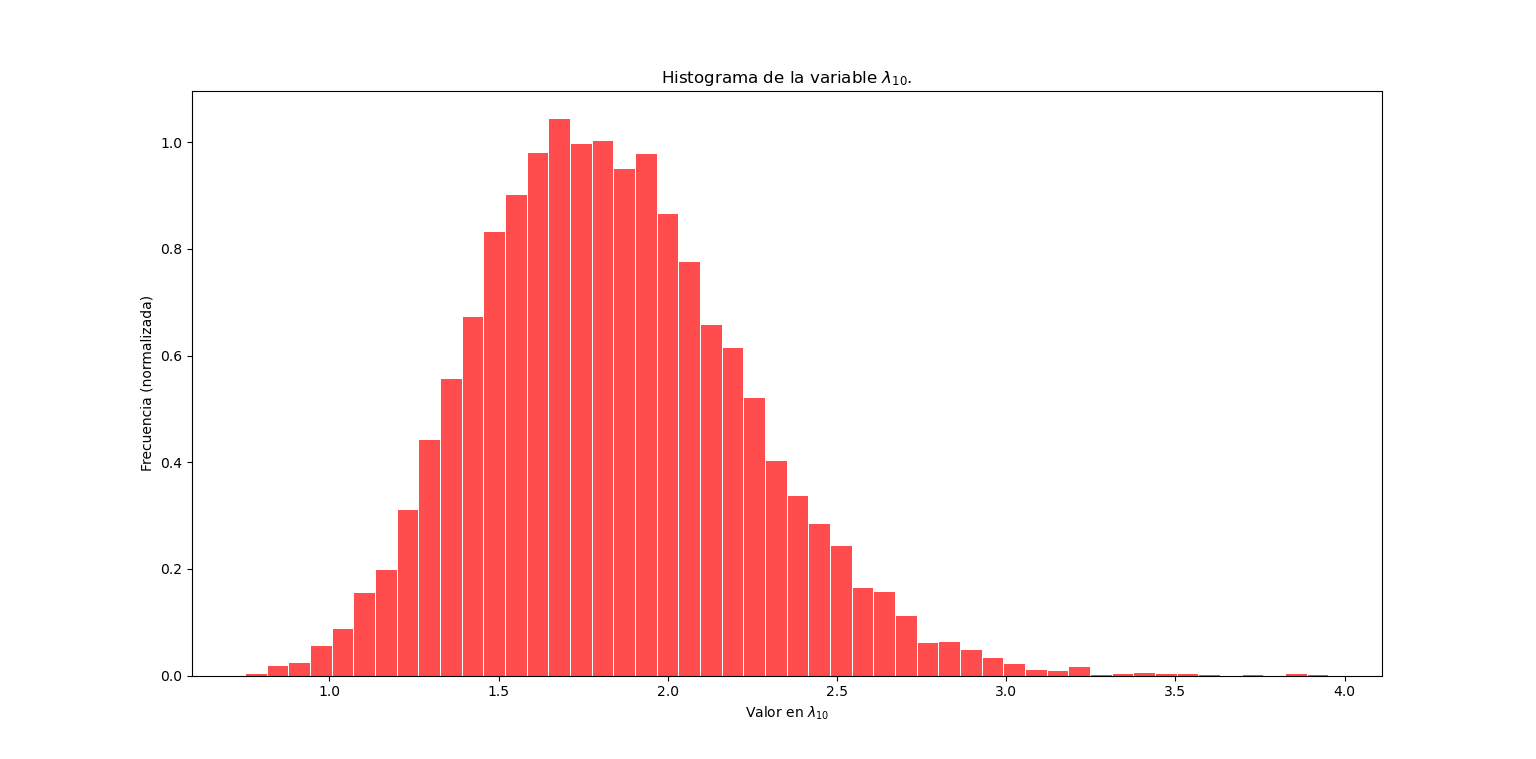
\includegraphics[width=\linewidth]{22.png}
        \caption{Histograma para $\lambda_{10}$}
    \end{figure} 
    \begin{figure}[h!]
        \centering
        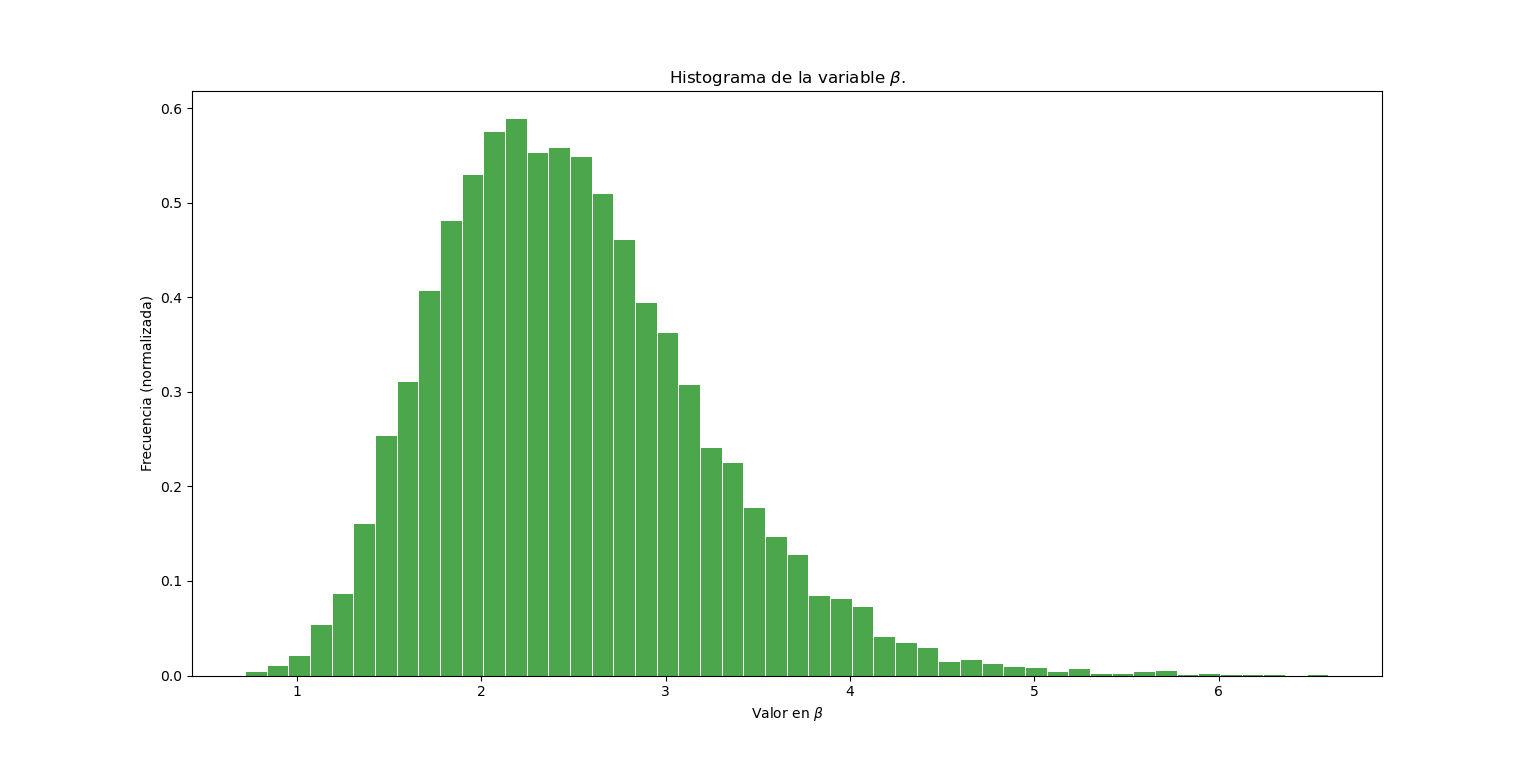
\includegraphics[width=\linewidth]{23.png}
        \caption{Histograma para $\beta$}
    \end{figure} 
    Ciertamente la cantidad de dimensiones del vector de parámetros vuelve más difícil
    la visualización de recorrido de la cadena, así como el estudio 
    de la densidad objetivo y por ende, del estudio de lo preciso de las simulaciones 
    hechas aquí, por lo que los resultados anteriores deben ser sujetos a un análisis más detallado para conocer qué tan 
    acertados son.\\

    Para concluir, comprobamos que en efecto las propuestas hechas antes corresponden 
    a Kerneles de Gibss. En efecto. Recordemos que $\overline{\lambda}_{-i}$ representa al conjunto de datos $\lambda_1,...,\lambda_n$, 
    pero con el $i-$ésimo dato suprimido. Utilizando que los parámetros $\lambda_i$ son independientes entre sí, calculamos:
    \[
        f(\lambda_i|\overline{\lambda}_{-i},\beta,\overline{t})=\frac{f(\overline{\lambda},\beta|\overline{t})}{f(\overline{\lambda}_{-i},\beta|\overline{t})}
        \propto\frac{\mathcal{L}(\overline{t}|\overline{\lambda},\beta)f(\lambda_1|\beta)\cdot...\cdot f(\lambda_n|\beta)f(\beta)}{\mathcal{L}(\overline{t}|\overline{\lambda}_{-i},\beta)f(\lambda_1|\beta)\cdot...\cdot f(\lambda_{i-1}|\beta)f(\lambda_{i+1}|\beta)\cdot...\cdot f(\lambda_{n}|\beta)f(\beta)}=\frac{\mathcal{L}(\overline{t}|\overline{\lambda},\beta)}{\mathcal{L}(\overline{t}|\overline{\lambda}_{-i},\beta)}f(\lambda_{i}|\beta).
    \]
    Y utilizando que $p_i\sim Poisson(\lambda_it_i)$, que $\lambda_i|\beta \sim Gamma(\alpha,\beta)$, y que los elementos $p_i$ y $t_i$ son, para nuestros propósitos, constantes,
    se tiene que 
    
    \begin{align*}
            \frac{\mathcal{L}(\overline{t}|\overline{\lambda},\beta)}{\mathcal{L}(\overline{t}|\overline{\lambda}_{-i},\beta)}f(\lambda_{i}|\beta)&=\left(\prod_{j=1}^{n}\frac{(\lambda_jt_j)^{p_j}e^{-\lambda_jt_j}}{p_j!}\right)\left(\prod_{j\neq i}\frac{(\lambda_jt_j)^{p_j}e^{-\lambda_jt_j}}{p_j!}\right)^{-1}\left(\frac{(\beta\lambda_i)^{\alpha-1}\beta e^{-\beta\lambda_i}}{\Gamma(\alpha)}\right)\\
            &=\frac{(\lambda_it_i)^{p_i}e^{-\lambda_it_t}}{p_i!}\left(\frac{(\beta\lambda_i)^{\alpha-1}\beta e^{-\beta\lambda_i}}{\Gamma(\alpha)}\right)\\
            &\propto \lambda_i^{p_i+\alpha-1}e^{-\lambda_i(t_i+\beta)}\\
            &\propto f_G(\lambda_i),
    \end{align*}
    donde $G\sim \Gamma(p_i+\alpha,t_i+\beta)$, por lo que 
    \[
    \lambda_i|\overline{\lambda}_{-i},\beta,\overline{t}\sim \Gamma(p_i+\alpha,t_i+\beta),
    \] 
    justo como buscábamos.

    Finalmente, en el caso de $\beta$, notamos que  
    \[
        f(\lambda_1,...,\lambda_n,\beta|\overline{p})\propto\mathcal{L}(\overline{p},\overline{\lambda},\beta)f(\lambda_1,...,\lambda_n,\beta)\propto f(\lambda_1|\beta)\cdot...\cdot f(\lambda_n|\beta)f(\beta), 
    \]
    y sabiendo $\lambda_i|\beta \sim Gamma(\alpha,\beta)$, y que $\beta\sim\Gamma(\gamma,\delta)$, usando los parámetros que no involucren $\beta$ como constantes, 
    se tiene que 
    \[
        f(\lambda_1,...,\lambda_n,\beta|\overline{p})\propto\frac{\beta^{n\alpha+\gamma-1} \delta^{\gamma}e^{-\beta(\sum_{i=1}^{n}\lambda_i+\delta)\prod_{i=1}^{n}\lambda_i^{\alpha-1}}}{\Gamma(\alpha)^{n}\Gamma(\gamma)}\propto \beta^{n\alpha+\gamma-1}e^{-\beta(\sum_{i=1}^{n}\lambda_i+\delta)},
    \]
    y esta última función es a su vez proporcional a la función de densidad de una variable $\Gamma(n\alpha+\gamma,\sum_{i=1}^{n}\lambda_i +\delta)$.
    Se concluye entonces que 
    \[
        \beta|\overline{\lambda},\overline{t}\sim \Gamma(n\alpha+\gamma,\sum_{i=1}^{n}+\delta).
    \]
    Se sigue que las propuestas anteriores son Kerneles Gibbs.
\end{itemize}
\end{document}